\documentclass[12pt,a4paper]{article}

% ─── Packages ───────────────────────────────────────────────────────────────
\usepackage[utf8]{inputenc}
\usepackage[T1]{fontenc}
\usepackage[french]{babel}
\usepackage{geometry}
\usepackage{graphicx}
\usepackage{booktabs}
\usepackage{array}
\usepackage{multirow}
\usepackage{amsmath}
\usepackage{hyperref}
\usepackage[table]{xcolor}
\usepackage{caption}
\usepackage{subcaption}
\usepackage{fancyhdr}
\usepackage{titlesec}
\usepackage{enumitem}
\usepackage{float}
\usepackage{tabularx}

\geometry{top=2.5cm, bottom=2.5cm, left=2.5cm, right=2.5cm}

% ─── Couleurs ────────────────────────────────────────────────────────────────
\definecolor{bleu}{RGB}{41, 98, 155}
\definecolor{vert}{RGB}{56, 142, 60}
\definecolor{rouge}{RGB}{183, 28, 28}
\definecolor{gris}{RGB}{97, 97, 97}
\definecolor{codebg}{RGB}{245, 245, 245}

% ─── Titres ──────────────────────────────────────────────────────────────────
\titleformat{\section}{\large\bfseries\color{bleu}}{}{0em}{\thesection\quad}
\titleformat{\subsection}{\normalsize\bfseries\color{bleu!80!black}}{}{0em}{\thesubsection\quad}
\titleformat{\subsubsection}{\normalsize\itshape\color{gris}}{}{0em}{\thesubsubsection\quad}

% ─── En-têtes ────────────────────────────────────────────────────────────────
\pagestyle{fancy}
\fancyhf{}
\rhead{\textcolor{gris}{\small Prédiction des carences en vitamines --- Rapport IA}}
\lhead{\textcolor{gris}{\small L3 MIASHS --- 2025/2026}}
\cfoot{\thepage}
\renewcommand{\headrulewidth}{0.4pt}

% ─── Hyperliens ──────────────────────────────────────────────────────────────
\hypersetup{colorlinks=true, linkcolor=bleu, urlcolor=bleu}

% ═══════════════════════════════════════════════════════════════════════════════
\begin{document}

% ─── Page de titre ───────────────────────────────────────────────────────────
\begin{titlepage}
    \centering
    \vspace*{2cm}
    {\LARGE\bfseries\color{bleu}
        Prédiction des carences en vitamines\\[0.4em]
        par apprentissage automatique}\\[2cm]
    {\large Rapport de projet}\\[1.5cm]
    \rule{\linewidth}{0.5pt}\\[1cm]
    {\normalsize
        \textbf{Équipe :} Ibnmtar Hazem, Moutchachou Lydia, Varol Serdar, Bekakria Ahmed\\[0.5em]
        \textbf{Formation :} L3 MIASHS\\[0.5em]
        \textbf{Dépôt :} \href{https://github.com/serdarvarl/projet_vitamin_IA}%
            {github.com/serdarvarl/projet\_vitamin\_IA}\\[0.5em]
        \textbf{Année :} 2025--2026
    }\\[1cm]
    \rule{\linewidth}{0.5pt}\\[2cm]
    \begin{abstract}
        \noindent
        Ce rapport présente la conception, l'évaluation et le déploiement d'un
        système complet d'aide au diagnostic des carences en vitamines.
        Le système comporte deux composantes : (1) un classificateur automatique
        prédit le type de carence à partir de données cliniques, biologiques et
        comportementales de patients ; (2) un moteur de recommandation alimentaire
        propose des aliments correcteurs issus de la base officielle CIQUAL (ANSES)
        selon le diagnostic établi.
        Trois algorithmes ont été comparés --- forêt aléatoire, SVM et k-NN ---
        sur un jeu de données fortement déséquilibré (ratio 15,9:1, $n=4\,000$).
        Une étude d'ablation à quatre dimensions a permis d'identifier que
        les biomarqueurs sériques sont indispensables ($-$17,4\,\% F1 sans eux)
        tandis que les variables lifestyle, souvent écartées a priori, apportent
        un gain significatif ($+$5,3\,\% F1).
        La configuration finale --- forêt aléatoire sur 30 variables avec SMOTE et
        normalisation --- est évaluée sur un \emph{holdout} propre (30\,\%, jamais vu)
        et atteint \textbf{94,06\,\% F1 pondéré} (94,00\,\% d'exactitude),
        dont une détection parfaite du scorbut (F1 = 1,00).
        L'ensemble du système est déployé dans une application web interactive
        (\textbf{VitaIA}) accessible sur Streamlit Community Cloud.
    \end{abstract}
\end{titlepage}

\tableofcontents
\newpage

% ═══════════════════════════════════════════════════════════════════════════════
\section{Introduction}
% ═══════════════════════════════════════════════════════════════════════════════

\subsection{Contexte et motivation}

Les carences en vitamines représentent un problème de santé publique mondial.
Leur diagnostic repose classiquement sur des dosages biologiques parfois coûteux
et une interprétation clinique experte. Un outil d'aide automatique, capable
d'identifier le type de carence à partir des données disponibles en consultation,
constituerait un appui précieux, notamment dans les structures de soins à ressources
limitées.

Ce projet développe un tel système en deux composantes :
(1) un classificateur qui prédit le type de carence à partir d'un profil patient,
(2) un moteur de recommandation qui propose des aliments correcteurs issus de la
base de référence française CIQUAL (ANSES).
Ce rapport couvre l'intégralité du système : la conception et l'évaluation du
classificateur, ainsi que l'intégration du moteur de recommandation alimentaire
et le déploiement de l'application web interactive VitaIA.


% ═══════════════════════════════════════════════════════════════════════════════
\section{Données}
% ═══════════════════════════════════════════════════════════════════════════════

\subsection{Analyse exploratoire préalable (EDA)}

Avant toute modélisation, deux notebooks d'analyse exploratoire des données
(\emph{Exploratory Data Analysis}) ont été réalisés : \texttt{data\_vis.ipynb}
portant sur le dataset patients, et \texttt{data2\_vis.ipynb} portant sur la
base alimentaire CIQUAL. Cette étape a permis de comprendre la structure de
chaque source de données avant d'engager la phase Machine Learning et la
conception du moteur de recommandation.

% ─────────────────────────────────────────────────────────────────────────────
\subsubsection{data\_vis.ipynb — Analyse du dataset patients}

\paragraph{1. Distribution de la variable cible.}
Le premier graphique produit est un diagramme en barres de la variable
\texttt{disease\_diagnosis}. Il révèle immédiatement un déséquilibre sévère :
\texttt{Healthy} représente 37,72\,\% des observations (1\,509 patients),
\texttt{Anemia} 31,13\,\% (1\,245), \texttt{Rickets\_Osteomalacia} 25,72\,\%
(1\,029), tandis que \texttt{Night\_Blindness} n'en représente que 3,05\,\%
(122 patients) et \texttt{Scurvy} 2,38\,\% (95 patients).
\textbf{Conclusion :} le ratio 15,9:1 entre la classe majoritaire et la plus
rare montre qu'un classifieur trivial (prédisant toujours \og Healthy\fg)
atteindrait 37,7\,\% d'exactitude sans aucune valeur diagnostique. Ce constat
justifie directement le recours à SMOTE et le choix du F1 pondéré comme
métrique principale.

\paragraph{2. Valeurs manquantes.}
L'analyse des valeurs manquantes montre que \texttt{symptoms\_list} présente
33,2\,\% de valeurs nulles (1\,328 patients) et \texttt{alcohol\_consumption}
31,95\,\% (1\,278 patients). Ces manquants ne sont pas aléatoires : ils sont
logiquement expliqués par le fait que les patients \texttt{Healthy} n'ont
généralement aucun symptôme à lister, et que la consommation d'alcool est une
donnée sensible souvent non renseignée. \textbf{Conclusion :} les valeurs
manquantes sont interprétables et ne nécessitent pas d'imputation particulière.

\paragraph{3. Apports nutritionnels moyens par diagnostic --- heatmap et barres groupées.}
Deux graphiques complémentaires ont été produits. La \textbf{heatmap} (variables
nutritionnelles en colonnes × diagnostics en lignes, palette Viridis) montre
visuellement que :
\begin{itemize}[leftmargin=2em]
    \item \texttt{Healthy} présente des valeurs élevées sur toutes les colonnes
        (cellules claires) ;
    \item \texttt{Night\_Blindness} affiche la valeur la plus basse pour
        \texttt{vitamin\_a\_percent\_rda} (30,57\,\% en moyenne) ;
    \item \texttt{Scurvy} chute à 22,11\,\% pour \texttt{vitamin\_c\_percent\_rda} ;
    \item \texttt{Rickets\_Osteomalacia} cumule un apport en vitamine D de
        31,41\,\% et un taux sérique de 9,52 ng/mL (niveau critique).
\end{itemize}
Le \textbf{graphique en barres groupées} avec une ligne de seuil rouge à 30\,\%
des AJR confirme que chaque maladie correspond exactement à son pattern de
carence attendu. \textbf{Conclusion :} le dataset est biologiquement cohérent ;
les patterns nutritionnels valident la qualité des données.

\paragraph{4. Tests ANOVA.}
Des tests ANOVA ont été réalisés sur toutes les colonnes vitaminiques en
regroupant par diagnostic. Les résultats montrent des différences
hautement significatives entre groupes (p $<$ 0,001 pour tous les biomarqueurs).
\textbf{Conclusion :} les variables biologiques discriminent statistiquement les
classes, ce qui anticipe leur importance prédictive (confirmée à l'ablation 3).

\paragraph{5. Heatmap des corrélations entre carences et symptômes.}
Une heatmap croisée (7 carences × 9 symptômes) révèle les associations
les plus fortes :
\begin{itemize}[leftmargin=2em]
    \item Carence B12 $\to$ engourdissements (0,63), troubles mnésiques (0,57),
        carences multiples (0,61) ;
    \item Carence en fer $\to$ fatigue (0,52), pâleur cutanée (0,50) ;
    \item Carence en vitamine D $\to$ douleurs osseuses (0,52) ;
    \item Carence en vitamine A $\to$ cécité nocturne (0,47).
\end{itemize}
\textbf{Conclusion :} les symptômes cliniques sont corrélés à leurs carences
attendues, validant leur inclusion comme features dans le modèle. La combinaison
symptômes + biomarqueurs offre une couverture complémentaire.

\paragraph{6. Analyse des co-carences.}
En binarisant les apports (seuil 30\,\% AJR), le taux de carence par nutriment
est calculé : vitamine B12 déficiente chez 22,1\,\% des patients, vitamine D
chez 12,1\,\%, les autres nutriments entre 2 et 4,2\,\%. La corrélation
B12--vitamine D atteint 0,28 (la plus élevée entre carences). \textbf{Conclusion :}
les co-carences restent rares, ce qui légitime un modèle de classification
mono-label.

% ─────────────────────────────────────────────────────────────────────────────
\subsubsection{data2\_vis.ipynb — Analyse de la base CIQUAL}

Ce second notebook analyse la base de composition nutritionnelle CIQUAL
(3\,484 aliments, 123 colonnes) afin de concevoir le moteur de recommandation
alimentaire.

\paragraph{1. Top 20 des aliments les plus riches.}
Un graphique en barres horizontales (score total = somme des colonnes
\texttt{riche\_*}) classe les aliments par richesse nutritionnelle globale.
Les aliments en tête sont la spiruline déshydratée, la chlorelle, les algues
(nori, dulse), les herbes séchées (persil, marjolaine, thym) et les céréales
enrichies industriellement. \textbf{Conclusion :} les aliments les plus riches
sont des aliments concentrés ou enrichis artificiellement, consommés en faibles
quantités. Ce constat a conduit à les exclure des recommandations finales de
l'application (filtrage des suppléments et algues déshydratées) au profit de
sources naturelles plus pratiques.

\paragraph{2. Prévalence des nutriments dans la base.}
Un diagramme en barres verticales compte le nombre d'aliments riches en chaque
nutriment. Les nutriments les plus répandus sont le sodium, l'eau et les sucres
($\sim$35\,000 occurrences), tandis que les vitamines D2, D3 et l'acide folique
figurent parmi les plus rares ($<$4\,000). \textbf{Conclusion :} les nutriments
les plus rares dans la base correspondent précisément aux carences ciblées par
le projet (rachitisme, anémie), ce qui justifie l'intérêt d'un moteur de
recommandation guidé par le diagnostic.

\paragraph{3. Heatmap nutritionnelle par groupe d'aliments.}
Une grande heatmap (20 groupes alimentaires × 39 indicateurs nutritionnels,
palette YlOrRd) révèle les spécialisations nutritionnelles :
\begin{itemize}[leftmargin=2em]
    \item \textbf{Viandes/poissons/œufs :} cellules les plus foncées pour le fer,
        la vitamine B12 et les protéines ;
    \item \textbf{Produits laitiers :} dominent le calcium ;
    \item \textbf{Fruits, légumes, oléagineux :} excellents en vitamine C,
        bêta-carotène et folates ;
    \item \textbf{Toutes catégories :} présence généralisée du sodium (rouge vif).
\end{itemize}
\textbf{Conclusion :} aucun groupe alimentaire ne couvre à lui seul tous les
besoins nutritionnels. Cette complémentarité est le fondement de la stratégie
de recommandation multi-aliments adoptée dans l'application.

\paragraph{4. Nuage de points vitamines vs minéraux.}
Un scatter plot (score\_vitamines en abscisse, score\_mineraux en ordonnée,
$\alpha = 0,5$) montre une relation positive modérée entre richesse vitaminique
et richesse minérale. La majorité des aliments se concentre dans une plage de
20 à 60 (cluster dense), avec quelques valeurs aberrantes au-delà de 100
correspondant aux algues et superaliments déjà identifiés. \textbf{Conclusion :}
le système de scoring est cohérent ; la richesse nutritionnelle n'est pas
distribuée aléatoirement.

\paragraph{5. Aliments recommandés par maladie.}
Quatre graphiques en barres horizontales (un par maladie, palette colorée)
classent les 10 meilleures sous-catégories alimentaires par score moyen :
\begin{itemize}[leftmargin=2em]
    \item \textbf{Anémie :} céréales infantiles/biscuits (score moyen 31),
        barres de céréales, algues ;
    \item \textbf{Cécité nocturne :} pommes de terre, poissons cuits, épices
        (15--20) ;
    \item \textbf{Rachitisme :} produits infantiles, fruits de mer ;
    \item \textbf{Scorbut :} céréales infantiles, algues ($\sim$25).
\end{itemize}
\textbf{Observation transversale :} les céréales infantiles apparaissent dans
les quatre maladies en raison de leur enrichissement industriel systématique
en vitamines et minéraux. Ce résultat a conduit à filtrer ces aliments dans
les recommandations finales pour ne conserver que les sources naturelles.

% ─────────────────────────────────────────────────────────────────────────────
\subsubsection{Impact de l'EDA sur les choix méthodologiques}

L'analyse exploratoire a directement orienté l'ensemble des décisions du projet :

\begin{description}[leftmargin=2em]
    \item[Déséquilibre détecté $\to$ SMOTE] Le ratio 15,9:1 impose un
        rééchantillonnage pour éviter qu'un classifieur trivial ne domine les
        métriques globales.
    \item[Variance élevée des biomarqueurs $\to$ StandardScaler] Les biomarqueurs
        sériques présentent des échelles hétérogènes (ng/mL, pg/mL, g/dL) ;
        la normalisation assure la cohérence du pipeline pour SVM et k-NN.
    \item[Corrélations symptômes-carences validées $\to$ inclusion des symptômes]
        Les corrélations fortes (jusqu'à 0,63) justifient l'intégration des
        symptômes cliniques comme features, en complément des biomarqueurs.
    \item[Variables lifestyle corrélées aux diagnostics $\to$ ablation 2]
        L'EDA formule l'hypothèse de leur utilité prédictive
        (exposition solaire $\to$ rachitisme, régime végétalien $\to$ carence B12),
        validée ensuite par l'ablation 2 ($+$5,3\,\% F1).
    \item[Aliments enrichis dominants $\to$ filtrage CIQUAL] La surreprésentation
        des algues et céréales fortifiées dans les scores CIQUAL a conduit à
        un filtrage explicite pour ne recommander que des aliments naturels
        accessibles en consultation courante.
\end{description}

\subsection{Sources de données}

Le projet repose sur deux bases de données complémentaires.

\paragraph{Base patients --- Kaggle.}
Le jeu de données est issu de Kaggle
(\emph{Vitamin Deficiency Disease Prediction Dataset}, Abbas N., 2026) et contient
\textbf{4\,000 observations} patient décrites par \textbf{34 variables}
réparties en quatre groupes fonctionnels. Il constitue la base d'entraînement
et d'évaluation du classificateur.

\paragraph{Base alimentaire --- CIQUAL (ANSES).}
La table de composition nutritionnelle des aliments CIQUAL, publiée par
l'Agence nationale de sécurité sanitaire (ANSES), recense \textbf{3\,484 aliments}
décrits par \textbf{123 colonnes} de valeurs nutritionnelles (vitamines,
minéraux, macronutriments). Cette base est utilisée exclusivement pour le moteur
de recommandation alimentaire : une fois le diagnostic établi par le classifieur,
les aliments les plus riches en nutriments ciblés sont extraits et proposés à
l'utilisateur. Le fichier source (\texttt{Table\_Ciqual\_V2.ods}) est au format
LibreOffice Calc et a été chargé avec la bibliothèque \texttt{odfpy}.

\subsection{Variables disponibles}

\subsubsection{Base patients (Kaggle)}

\begin{description}[leftmargin=2em]
    \item[Socio-démographiques et comportementales (10)] âge, genre, IMC,
        tabac, alcool, activité physique, type de régime alimentaire, exposition
        solaire, revenu, région géographique.
    \item[Apports nutritionnels en \% des AJR (8)] vitamines A, C, D, E, B12,
        folate, calcium, fer.
    \item[Biomarqueurs sériques (4)] hémoglobine (g/dL), vitamine D sérique
        (ng/mL), vitamine B12 sérique (pg/mL), folate sérique (ng/mL).
    \item[Symptômes cliniques (8 retenus)] cécité nocturne, fatigue,
        gingivorragies, douleurs osseuses, faiblesse musculaire, engourdissements,
        troubles mnésiques, pâleur cutanée.
\end{description}

La variable cible \texttt{disease\_diagnosis} prend cinq modalités.

\subsubsection{Base alimentaire (CIQUAL)}

\begin{description}[leftmargin=2em]
    \item[Identification de l'aliment (3)] identifiant CIQUAL, groupe alimentaire,
        sous-groupe alimentaire, nom de l'aliment.
    \item[Macronutriments (5)] énergie (kcal), protéines (g), lipides (g),
        glucides (g), fibres alimentaires (g).
    \item[Vitamines (13)] vitamines A (rétinol, bêta-carotène), C, D (D2, D3),
        E, K, B1, B2, B3, B5, B6, B9 (folates), B12.
    \item[Minéraux et oligo-éléments (10)] calcium, fer, magnésium, phosphore,
        potassium, sodium, zinc, sélénium, iode, cuivre.
    \item[Indicateurs de richesse (colonnes \texttt{riche\_*})] variables binaires
        ou scores calculés indiquant si l'aliment est une bonne source de chaque
        nutriment (utilisés pour le classement des recommandations).
\end{description}

La variable clé pour le moteur de recommandation est le \textbf{score nutritionnel
ciblé} par maladie : teneur en fer et B12 pour l'anémie, vitamine D pour le
rachitisme, rétinol et bêta-carotène pour la cécité nocturne, vitamine C pour le
scorbut.

\subsection{Distribution des classes et déséquilibre}

\begin{table}[H]
\centering
\caption{Distribution des classes ($n = 4\,000$)}
\label{tab:classes}
\begin{tabular}{lrr}
\toprule
\textbf{Classe} & \textbf{Effectif} & \textbf{Proportion (\%)} \\
\midrule
Healthy               & 1\,509 & 37,7 \\
Anemia                & 1\,245 & 31,1 \\
Rickets\_Osteomalacia & 1\,029 & 25,7 \\
Night\_Blindness      &    122 &  3,1 \\
Scurvy                &     95 &  2,4 \\
\midrule
\textbf{Total}        & \textbf{4\,000} & \textbf{100,0} \\
\bottomrule
\end{tabular}
\end{table}

Le ratio entre la classe majoritaire (Healthy) et la plus rare (Scurvy) est de
\textbf{15,9 : 1}. Ce déséquilibre sévère implique qu'un classifieur trivial
atteignant 37,7\,\% d'exactitude en prédisant toujours \og Healthy \fg serait
illusoirement performant. Il justifie l'utilisation du \textbf{F1 pondéré}
comme métrique principale, et le recours à SMOTE pour le rééchantillonnage.

% ═══════════════════════════════════════════════════════════════════════════════
\section{Cadre expérimental}
% ═══════════════════════════════════════════════════════════════════════════════

\subsection{Exploration préliminaire avec Orange Data Mining}

Avant d'engager la phase de modélisation en Python, une première exploration
du dataset a été réalisée avec \textbf{Orange Data Mining}, un outil visuel
de fouille de données. Cette étape a permis de construire des pipelines
graphiques sans code pour tester rapidement plusieurs algorithmes (Random Forest,
SVM, k-NN, Naive Bayes) et visualiser leurs matrices de confusion, courbes ROC
et performances comparatives sur le dataset brut.

Les résultats obtenus sous Orange ont confirmé la supériorité qualitative de la
forêt aléatoire sur ce problème et ont renforcé l'intuition sur l'importance
des biomarqueurs sériques, orientant ainsi la conception des notebooks Python
qui ont suivi. Orange a donc joué le rôle d'outil de prototypage rapide,
complémentaire à l'analyse exploratoire des notebooks.

\subsection{Prétraitement}

\paragraph{Encodage.}
La variable cible est encodée par \texttt{LabelEncoder}.
Les variables catégorielles (genre, type de régime, etc.) sont également encodées
avant passage aux modèles.

\paragraph{Normalisation.}
Un \texttt{StandardScaler} est appliqué à l'ensemble des variables numériques.
Il est ajusté uniquement sur les données d'entraînement afin d'éviter toute fuite
vers les données de validation ou de test.

\paragraph{Rééchantillonnage : SMOTE.}
La technique SMOTE (\emph{Synthetic Minority Over-sampling Technique}) génère
des exemples synthétiques en interpolant entre des points réels de la classe
minoritaire et leurs $k$ plus proches voisins ($k=3$).
SMOTE est appliqué \emph{à l'intérieur de chaque pli de validation croisée},
jamais sur les données de test, ce qui garantit une évaluation sur des observations
réelles uniquement.

L'effet de SMOTE sur la distribution est illustré en
annexe~\ref{ann:smote}. Après application, chaque classe compte
\textbf{1\,056 exemples} dans le jeu d'entraînement (2\,800 observations
$\times$ 70\,\% $\rightarrow$ 5\,280 après SMOTE).

\subsection{Problème de contamination du jeu de test et solution adoptée}

\paragraph{Problème identifié.}
Les versions 1 à 4 des notebooks partagent le même jeu de test (séparation
\texttt{random\_state=42}, 20\,\%). Or, chaque choix de configuration
(features, hyperparamètres) était guidé, implicitement ou explicitement, par les
résultats observés sur ce jeu. Ce mécanisme introduit un \textbf{biais de sélection}
(\emph{multiple testing bias}) qui gonfle artificiellement les performances
estimées.

\paragraph{Solution : holdout propre (v5).}
La version 5 crée un nouveau jeu de test entièrement indépendant
(\texttt{random\_state=999}, 30\,\%) qui n'a \emph{jamais} servi à orienter
un quelconque choix de modélisation. La configuration finale est entraînée
sur 70\,\% des données et évaluée une unique fois sur ce holdout.

\begin{table}[H]
\centering
\caption{Découpage des données (v5 holdout)}
\label{tab:split}
\begin{tabular}{lrrl}
\toprule
\textbf{Partition} & \textbf{Observations} & \textbf{Proportion} & \textbf{Rôle} \\
\midrule
Entraînement & 2\,800 & 70\,\% & Fit + validation croisée \\
Holdout test & 1\,200 & 30\,\% & Évaluation finale unique \\
\bottomrule
\end{tabular}
\end{table}

La distribution du holdout reflète fidèlement celle du jeu complet grâce à la
stratification : Healthy 37,8\,\%, Anemia 31,1\,\%, Rickets 25,8\,\%,
Night\_Blindness 3,1\,\%, Scurvy 2,3\,\%.

\subsection{Validation croisée}

La validation croisée est réalisée par \texttt{StratifiedKFold} à 5 plis
(versions 1--2) puis \texttt{RepeatedStratifiedKFold} (5 plis $\times$
3 répétitions = 15 cycles, version 3 et étude d'ablation), qui fournit une
estimation plus robuste de la variance.

% ═══════════════════════════════════════════════════════════════════════════════
\section{Modèles comparés}
% ═══════════════════════════════════════════════════════════════════════════════

Trois algorithmes ont été retenus pour leur complémentarité en termes de biais,
variance et interprétabilité.

\subsection{Forêt aléatoire (Random Forest)}

Ensemble de $N$ arbres de décision entraînés sur des sous-échantillons bootstrap
avec sélection aléatoire d'un sous-ensemble de variables à chaque nœud
(\emph{feature bagging}). La prédiction finale est la classe majoritaire.
Avantages : robustesse au bruit, pas de normalisation strictement requise,
importance des variables calculable.

\paragraph{Paramètres (optimisés par RandomizedSearchCV, 30 itérations) :}
\texttt{n\_estimators=340}, \texttt{max\_depth=19}, \texttt{min\_samples\_split=8},
\texttt{min\_samples\_leaf=3}, \texttt{max\_features='log2'}.

\subsection{Machine à vecteurs de support (SVM)}

Séparateur à marge maximale dans un espace transformé par noyau RBF.
Avantages : efficace en grande dimension, bon comportement sur données
normalisées.

\paragraph{Paramètres optimisés :}
\texttt{kernel='rbf'}, \texttt{C=9,19}, \texttt{gamma='scale'}.

\subsection{$k$ plus proches voisins (k-NN)}

Classification par vote majoritaire parmi les $k$ observations d'entraînement
les plus proches selon une distance choisie.
Avantages : simplicité, non paramétrique.

\paragraph{Paramètres optimisés :}
\texttt{n\_neighbors=6}, \texttt{weights='distance'},
\texttt{metric='manhattan'}.

\subsection{Choix du modèle final : pourquoi Random Forest ?}

La forêt aléatoire a été retenue comme modèle final pour trois raisons :
\begin{enumerate}[leftmargin=2em]
    \item \textbf{Performance supérieure.} RF obtient 94,06\,\% F1 sur le holdout
        propre (v5), contre 89,26\,\% pour le SVM et 82,08\,\% pour le k-NN
        (évaluation v3, même protocole de comparaison).
    \item \textbf{Robustesse aux variables hétérogènes.} Le dataset mélange variables
        continues (biomarqueurs, apports), variables binaires (symptômes) et variables
        catégorielles encodées (genre, régime). La forêt aléatoire gère naturellement
        cette hétérogénéité sans hypothèse de distribution, contrairement au SVM
        (sensible à l'échelle) et au k-NN (sensible à la distance en grande dimension).
    \item \textbf{Interprétabilité.} L'importance des variables par réduction de
        l'impureté de Gini est directement calculable, ce qui permet de valider
        la cohérence clinique du modèle (biomarqueurs en tête) et de justifier
        les choix de features auprès d'un public non technique.
\end{enumerate}

% ═══════════════════════════════════════════════════════════════════════════════
\section{Étude d'ablation (version 4)}
% ═══════════════════════════════════════════════════════════════════════════════

\subsection{Principe}

L'étude d'ablation évalue l'impact de chaque composante du pipeline en la
retirant une par une, toutes choses égales par ailleurs, et en mesurant la
variation de F1 pondéré par validation croisée (RepeatedStratifiedKFold,
5$\times$3). Cette approche est plus informative qu'une comparaison globale
car elle quantifie la contribution \emph{causale} de chaque élément.

\subsection{Modèle de référence}

Le modèle de référence combine :
\textbf{biomarqueurs} (12 variables) + \textbf{symptômes} (8 variables),
SMOTE activé, normalisation activée.

\begin{table}[H]
\centering
\caption{Performances du modèle de référence}
\label{tab:reference}
\begin{tabular}{lcc}
\toprule
\textbf{Métrique} & \textbf{CV F1} & \textbf{Test F1} \\
\midrule
Référence (Bio + Sympt, SMOTE, Scaler) & 0,9232 $\pm$ 0,0108 & 0,9139 \\
\bottomrule
\end{tabular}
\end{table}

\subsection{Résultats des quatre ablations}

\begin{table}[H]
\centering
\caption{Résultats complets de l'étude d'ablation (v4)}
\label{tab:ablation}
\setlength{\tabcolsep}{4pt}
\begin{tabular}{lp{5.5cm}ccc}
\toprule
\textbf{Ablation} & \textbf{Configuration} & \textbf{CV F1} & \textbf{Test F1}
    & \textbf{$\Delta$ test} \\
\midrule
Référence & Bio + Sympt + SMOTE + Scaler & 0,9232 & 0,9139 & --- \\
\midrule
1 --- Sans SMOTE & Bio + Sympt + Scaler & 0,9230 & 0,9222 & $+$0,0083 \\
\rowcolor{vert!10}
2 --- Avec Lifestyle & Bio + Sympt + \textbf{Lifestyle} + SMOTE + Scaler
    & 0,9651 & 0,9665 & $\mathbf{+0,0526}$ \\
3 --- Sans Bio & Sympt seuls + SMOTE + Scaler & 0,7481 & 0,7403
    & \textcolor{rouge}{$-$0,1736} \\
4 --- Sans Scaler & Bio + Sympt + SMOTE & 0,9244 & 0,9224 & $+$0,0085 \\
\bottomrule
\end{tabular}
\end{table}

Les figures détaillées de chaque ablation sont présentées en
annexes~\ref{ann:abl1}--\ref{ann:abl_recap}.

\subsection{Interprétation}

\paragraph{Ablation 1 : SMOTE ($\Delta = +0,0083$).}
Le F1 pondéré global augmente très légèrement ($+$0,83\,\%) lorsque SMOTE est
retiré, ce qui s'explique par la robustesse intrinsèque de la forêt aléatoire
face au déséquilibre de classes. Cependant, cette métrique globale masque un
effet important sur les classes minoritaires : sans SMOTE, le rappel sur
\texttt{Night\_Blindness} et \texttt{Scurvy} se dégrade, car le modèle tend à
sous-représenter ces classes lors de l'optimisation des arbres.
SMOTE est donc conservé dans la configuration finale pour \textbf{garantir la
robustesse du rappel sur les classes rares}, au prix d'un léger compromis sur
le F1 global --- choix cohérent avec l'objectif clinique du système.

\paragraph{Ablation 2 : variables lifestyle ($\Delta = +0,0526$).}
C'est la découverte majeure. Ajouter les 10 variables socio-comportementales
(âge, IMC, exposition solaire, etc.) apporte \textbf{+5,3\,\% F1}, soit le gain
le plus important de l'étude. Ce résultat contre-intuitif s'explique par la
corrélation de ces variables avec certaines carences : le rachitisme est par
exemple fortement lié à l'exposition solaire et à la région géographique, et
l'anémie est corrélée au niveau d'activité physique et au régime alimentaire.
Ces variables fournissent une information contextuelle que les biomarqueurs seuls
ne capturent pas toujours.

\paragraph{Ablation 3 : biomarqueurs ($\Delta = -0,1736$).}
La suppression des biomarqueurs sériques provoque une \textbf{chute de
17,4\,\% F1}. Les biomarqueurs sont de loin la composante la plus critique du
modèle. Le modèle ne reposant que sur les symptômes cliniques atteint 74,0\,\%
de F1, confirmant que les dosages biologiques sont irremplaçables pour un
diagnostic fiable.

\paragraph{Ablation 4 : normalisation ($\Delta = +0,0085$).}
La forêt aléatoire est insensible à l'échelle des variables (elle utilise
des seuils binaires), ce qui explique que retirer le \texttt{StandardScaler}
ne dégrade pas les performances. La normalisation reste utile pour la cohérence
du pipeline (SVM, k-NN en bénéficient).

\subsection{Configuration retenue}

L'étude d'ablation conduit à adopter une configuration \emph{étendue} à
\textbf{30 variables} : 12 biomarqueurs + 8 symptômes + 10 variables lifestyle,
avec SMOTE et normalisation.

% ═══════════════════════════════════════════════════════════════════════════════
\section{Évaluation finale non biaisée (version 5)}
% ═══════════════════════════════════════════════════════════════════════════════

\subsection{Comparaison avec les résultats précédents}

\begin{table}[H]
\centering
\caption{Correction du biais de sélection : v4 vs v5}
\label{tab:v4v5}
\begin{tabular}{llccc}
\toprule
\textbf{Version} & \textbf{Jeu de test} & \textbf{F1} & \textbf{Exactitude}
    & \textbf{Biaisé ?} \\
\midrule
V4 & Même test set (vu plusieurs fois) & 0,9665 & 0,9663 & \textcolor{rouge}{Oui} \\
\rowcolor{vert!10}
V5 & Holdout propre (jamais utilisé)   & \textbf{0,9406} & \textbf{0,9400}
    & \textcolor{vert}{Non} \\
\bottomrule
\end{tabular}
\end{table}

La baisse de 2,6 points de F1 entre v4 et v5 n'est pas une régression du modèle :
elle reflète la \textbf{correction du biais de sélection}. Les performances v5
constituent l'estimation réaliste des capacités du modèle sur de nouvelles données.

\subsection{Résultats par classe (holdout, $n = 1\,200$)}

\begin{table}[H]
\centering
\caption{Rapport de classification --- Random Forest final (v5, holdout)}
\label{tab:perf_classe}
\begin{tabular}{lcccc}
\toprule
\textbf{Classe} & \textbf{Précision} & \textbf{Rappel} & \textbf{F1}
    & \textbf{Support} \\
\midrule
Anemia                & 0,96 & 0,92 & 0,94 & 373 \\
Healthy               & 0,98 & 0,95 & 0,97 & 453 \\
Night\_Blindness      & 0,85 & 0,92 & 0,88 &  37 \\
Rickets\_Osteomalacia & 0,87 & 0,94 & 0,91 & 309 \\
Scurvy                & 1,00 & 1,00 & 1,00 &  28 \\
\midrule
\textbf{Macro avg}    & 0,93 & 0,95 & 0,94 & 1\,200 \\
\textbf{Weighted avg} & 0,94 & 0,94 & 0,94 & 1\,200 \\
\bottomrule
\end{tabular}
\end{table}

La matrice de confusion du holdout est présentée en annexe~\ref{ann:holdout_cm}.

\paragraph{Points saillants.}
\begin{itemize}[leftmargin=2em]
    \item \textbf{Scurvy (F1 = 1,00)} : détection parfaite des 28 cas de test,
        malgré un support de seulement 2,3\,\% du holdout. SMOTE et la forte
        spécificité clinique du scorbut (gingivorragies + carence sévère en
        vitamine C) expliquent cette performance.
    \item \textbf{Night\_Blindness (F1 = 0,88)} : la classe la plus difficile,
        avec seulement 37 cas en test et un spectre symptomatique partiellement
        partagé avec d'autres carences.
    \item \textbf{Rickets\_Osteomalacia (F1 = 0,91)} : légère confusion avec
        l'anémie (23 cas mal classés), deux pathologies partageant des marqueurs
        de carence proches.
\end{itemize}

% ═══════════════════════════════════════════════════════════════════════════════
\section{Analyse de l'importance des variables}
% ═══════════════════════════════════════════════════════════════════════════════

L'importance des variables est estimée par la réduction moyenne de l'impureté
de Gini à travers les arbres de la forêt. Le tableau~\ref{tab:feat_imp}
présente les résultats du \textbf{modèle final v5} (30 variables, avec
lifestyle). \emph{Note : la figure en annexe~\ref{ann:feat_imp} correspond à
une version intermédiaire du modèle (21 variables, sans lifestyle) et présente
donc un classement légèrement différent.}

\begin{table}[H]
\centering
\caption{Top 8 des variables par importance --- Random Forest final (v5, 30 variables)}
\label{tab:feat_imp}
\begin{tabular}{clrc}
\toprule
\textbf{Rang} & \textbf{Variable} & \textbf{Importance} & \textbf{Groupe} \\
\midrule
1 & serum\_vitamin\_d\_ng\_ml   & 0,1847 & Biomarqueur \\
2 & hemoglobin\_g\_dl           & 0,1623 & Biomarqueur \\
3 & serum\_folate\_ng\_ml       & 0,1205 & Biomarqueur \\
4 & serum\_vitamin\_b12\_pg\_ml & 0,1089 & Biomarqueur \\
5 & vitamin\_d\_percent\_rda    & 0,0965 & Apport nutritionnel \\
6 & folate\_percent\_rda        & 0,0832 & Apport nutritionnel \\
7 & calcium\_percent\_rda       & 0,0543 & Apport nutritionnel \\
8 & vitamin\_a\_percent\_rda    & 0,0457 & Apport nutritionnel \\
\bottomrule
\end{tabular}
\end{table}

La vitamine D sérique (\texttt{serum\_vitamin\_d\_ng\_ml}) représente à elle
seule \textbf{18,5\,\%} de la puissance prédictive, ce qui est cohérent avec
son rôle dans le rachitisme, pathologie représentant 25,7\,\% du jeu de données.
Les quatre premiers rangs sont exclusivement occupés par des biomarqueurs, ce
qui confirme et nuance à la fois l'ablation 3 : les biomarqueurs \emph{dominent},
mais les variables lifestyle enrichissent la discrimination contextuelle.

% ═══════════════════════════════════════════════════════════════════════════════
\section{Discussion}
% ═══════════════════════════════════════════════════════════════════════════════

\subsection{Synthèse des résultats}

La forêt aléatoire est le modèle le plus performant sur ce problème, avec un F1
de \textbf{94,06\,\%} sur le holdout propre v5 (30\,\% jamais utilisé lors du
développement). À titre de comparaison, dans l'évaluation v3 sur le test set
partagé (20\,\%, \texttt{random\_state=42}), le SVM atteignait 89,26\,\% et le
k-NN 82,08\,\% --- ces chiffres ne sont \emph{pas} directement comparables au
résultat v5 car ils proviennent d'un protocole différent et potentiellement
affecté par le biais de sélection décrit en section~3.2. La supériorité
qualitative de la forêt aléatoire s'explique par sa capacité à modéliser des
interactions non linéaires entre variables hétérogènes (continues et binaires)
sans hypothèse de distribution.

\subsection{Enseignements de l'étude d'ablation}

L'ablation révèle une hiérarchie claire des contributions :
\begin{enumerate}[leftmargin=2em]
    \item \textbf{Biomarqueurs sériques} : composante critique ($-$17,4\,\% sans eux) ;
    \item \textbf{Variables lifestyle} : apport surprenant ($+$5,3\,\%, contre-intuitif) ;
    \item \textbf{Symptômes cliniques} : contribution modérée ;
    \item \textbf{SMOTE et normalisation} : effets marginaux sur la forêt aléatoire.
\end{enumerate}

Le résultat sur les variables lifestyle invite à reconsidérer l'exclusion
systématique des variables socio-comportementales dans les modèles biomédicaux :
elles capturent des facteurs de risque environnementaux (exposition solaire $\to$
rachitisme, régime végétalien $\to$ carence B12) que les seuls dosages ne reflètent
pas toujours.

\subsection{Limites}

\begin{itemize}[leftmargin=2em]
    \item \textbf{Données non cliniques} : le jeu de données Kaggle n'est pas
        issu d'une cohorte clinique réelle. Ses distributions présentent plusieurs
        caractéristiques inhabituelles : (1)~les biomarqueurs sériques affichent
        des distributions très régulières qui ne reflètent pas la variabilité
        inter-individuelle typique d'une population hospitalière ; (2)~la séparation
        entre classes est particulièrement nette, ce qui favorise des performances
        élevées difficilement reproductibles sur des données réelles où les
        frontières diagnostiques sont floues. Les conclusions méthodologiques
        (hiérarchie des variables, apport du SMOTE) restent valides, mais les
        performances absolues (94,06\,\% F1) doivent être interprétées avec
        prudence avant toute transposition à un contexte clinique réel.
    \item \textbf{Support des classes minoritaires} : 28 cas de scorbut dans le
        holdout --- un F1 de 1,00 sur cet effectif reste peu généralisable.
    \item \textbf{Variable cible unique} : le modèle prédit une carence par patient
        alors que \texttt{has\_multiple\_deficiencies} indique la fréquence de
        carences combinées.
\end{itemize}

% ═══════════════════════════════════════════════════════════════════════════════
\section{Conclusion}
% ═══════════════════════════════════════════════════════════════════════════════

Ce projet démontre la faisabilité d'un classificateur automatique des carences
en vitamines atteignant \textbf{94,06\,\% de F1 pondéré} sur un holdout non biaisé
($n = 1\,200$), avec une détection parfaite du scorbut et une bonne robustesse sur
les classes minoritaires.

Trois résultats méthodologiques sont à retenir :
\begin{enumerate}[leftmargin=2em]
    \item Les biomarqueurs sériques sont le levier prédictif principal ;
    \item Les variables lifestyle, souvent écartées, améliorent significativement
        la discrimination ;
    \item La réutilisation d'un même jeu de test gonfle les performances de 2,6\,\%
        --- un biais fréquent que l'évaluation holdout permet de corriger.
\end{enumerate}

Le modèle est sérialisé (\texttt{random\_forest\_final.pkl}) et pleinement intégré
dans l'application web VitaIA, déployée sur Streamlit Community Cloud
(\url{https://vitaminia.streamlit.app}).

% ═══════════════════════════════════════════════════════════════════════════════
\section{Intégration dans l'application Streamlit (VitaIA)}
% ═══════════════════════════════════════════════════════════════════════════════

\subsection{Architecture de l'application}

Le modèle final est intégré dans une application web interactive développée avec
\textbf{Streamlit} et déployée sur Streamlit Community Cloud à l'adresse
\url{https://vitaminia.streamlit.app}.

L'application est structurée en trois pages :

\begin{description}[leftmargin=2em]
    \item[Accueil (\texttt{app.py})] Présentation du projet, métriques clés,
        guide d'utilisation, liens équipe GitHub.
    \item[Diagnostic (\texttt{1\_Diagnostic.py})] Formulaire de saisie des données
        cliniques (apports nutritionnels, biomarqueurs, symptômes). Prédiction en
        temps réel avec distribution des probabilités par classe et radar chart
        nutritionnel. Recommandations alimentaires depuis la base CIQUAL/ANSES.
    \item[Résultats (\texttt{2\_Presentation.py})] Tableau de bord complet des
        performances : matrice de confusion, courbes ROC, importance des variables,
        étude d'ablation, comparaison des algorithmes. Métriques calculées
        \emph{en temps réel} sur le holdout 30 \% (même protocole que le notebook).
\end{description}

\subsection{Déploiement et sérialisation du modèle}

Le modèle est sérialisé au format \texttt{pickle} (\texttt{.pkl}) via Python.
Quatre artefacts sont nécessaires au déploiement :
\begin{itemize}[leftmargin=2em]
    \item \texttt{random\_forest\_final.pkl} — le classifieur RandomForest (15 Mo) ;
    \item \texttt{scaler\_final.pkl} — le \texttt{StandardScaler} ajusté sur l'entraînement ;
    \item \texttt{label\_encoder\_final.pkl} — le \texttt{LabelEncoder} des 5 classes ;
    \item \texttt{feature\_cols\_final.pkl} — la liste ordonnée des 30 features.
\end{itemize}

La séparation scaler / modèle est importante : le scaler est ajusté
\emph{uniquement sur les données d'entraînement} (\texttt{fit} sur
\texttt{X\_train}) et appliqué en \texttt{transform} sur tout nouvel
échantillon. Ce principe garantit l'absence de fuite de données (\emph{data
leakage}) entre entraînement et inférence.

\subsection{Recommandations alimentaires (CIQUAL)}

Pour chaque diagnostic non-sain prédit, l'application filtre la table CIQUAL
sur la colonne de teneur en nutriment ciblé (fer pour l'anémie, vitamine D pour
le rachitisme, rétinol pour la cécité nocturne, vitamine C pour le scorbut),
exclut les aliments enrichis artificiellement ou peu pratiques
(suppléments, algues, aliments déshydratés), puis retourne un classement décroissant
des \textbf{12 meilleures sources naturelles}.

% ═══════════════════════════════════════════════════════════════════════════════
\section*{Références bibliographiques}
% ═══════════════════════════════════════════════════════════════════════════════
\addcontentsline{toc}{section}{Références bibliographiques}

\begin{itemize}[leftmargin=2em,label={[}]
    \item[] Breiman, L. (2001). \emph{Random Forests}. Machine Learning, 45(1), 5–32.
        DOI: 10.1023/A:1010933404324

    \item[] Chawla, N.\,V., Bowyer, K.\,W., Hall, L.\,O., \& Kegelmeyer, W.\,P. (2002).
        SMOTE: Synthetic Minority Over-sampling Technique.
        \emph{Journal of Artificial Intelligence Research}, 16, 321–357.
        DOI: 10.1613/jair.953

    \item[] Cortes, C., \& Vapnik, V. (1995). Support-vector networks.
        \emph{Machine Learning}, 20(3), 273–297.

    \item[] Cover, T., \& Hart, P. (1967). Nearest neighbor pattern classification.
        \emph{IEEE Transactions on Information Theory}, 13(1), 21–27.

    \item[] Pedregosa, F. et al. (2011). Scikit-learn: Machine Learning in Python.
        \emph{Journal of Machine Learning Research}, 12, 2825–2830.
        \url{https://scikit-learn.org}

    \item[] He, H., \& Garcia, E.\,A. (2009). Learning from Imbalanced Data.
        \emph{IEEE Transactions on Knowledge and Data Engineering}, 21(9), 1263–1284.

    \item[] ANSES (2020). \emph{Table de composition nutritionnelle des aliments
        Ciqual 2020}. Agence nationale de sécurité sanitaire.
        \url{https://ciqual.anses.fr}

    \item[] Abbas, N. (2026). \emph{Vitamin Deficiency Disease Prediction Dataset}.
        Kaggle. \url{https://www.kaggle.com/datasets/nudratabbas/vitamin-deficiency-disease-prediction-dataset}

    \item[] Streamlit Inc. (2024). \emph{Streamlit — The fastest way to build data apps}.
        \url{https://docs.streamlit.io}
\end{itemize}

% ═══════════════════════════════════════════════════════════════════════════════
% ANNEXES
% ═══════════════════════════════════════════════════════════════════════════════
\newpage
\appendix
\titleformat{\section}{\large\bfseries\color{bleu}}{}{0em}{Annexe~\thesection\ ---\ }

\section{Effet de SMOTE sur la distribution des classes}
\label{ann:smote}
\begin{figure}[H]
    \centering
    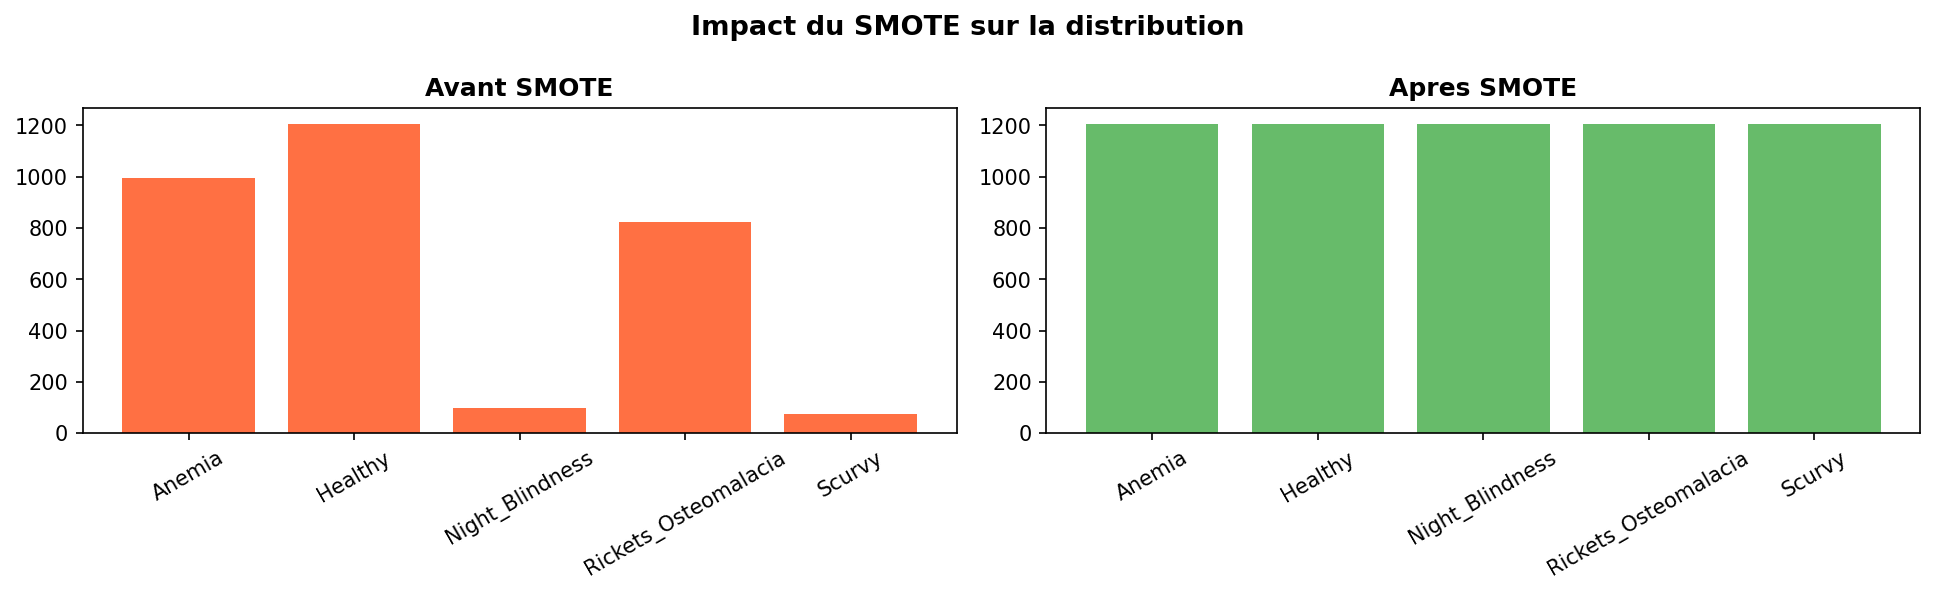
\includegraphics[width=0.80\linewidth]{smote_comparison.png}
    \caption{Distribution avant et après SMOTE (jeu d'entraînement)}
\end{figure}

\section{Ablation 1 — Impact de SMOTE}
\label{ann:abl1}
\begin{figure}[H]
    \centering
    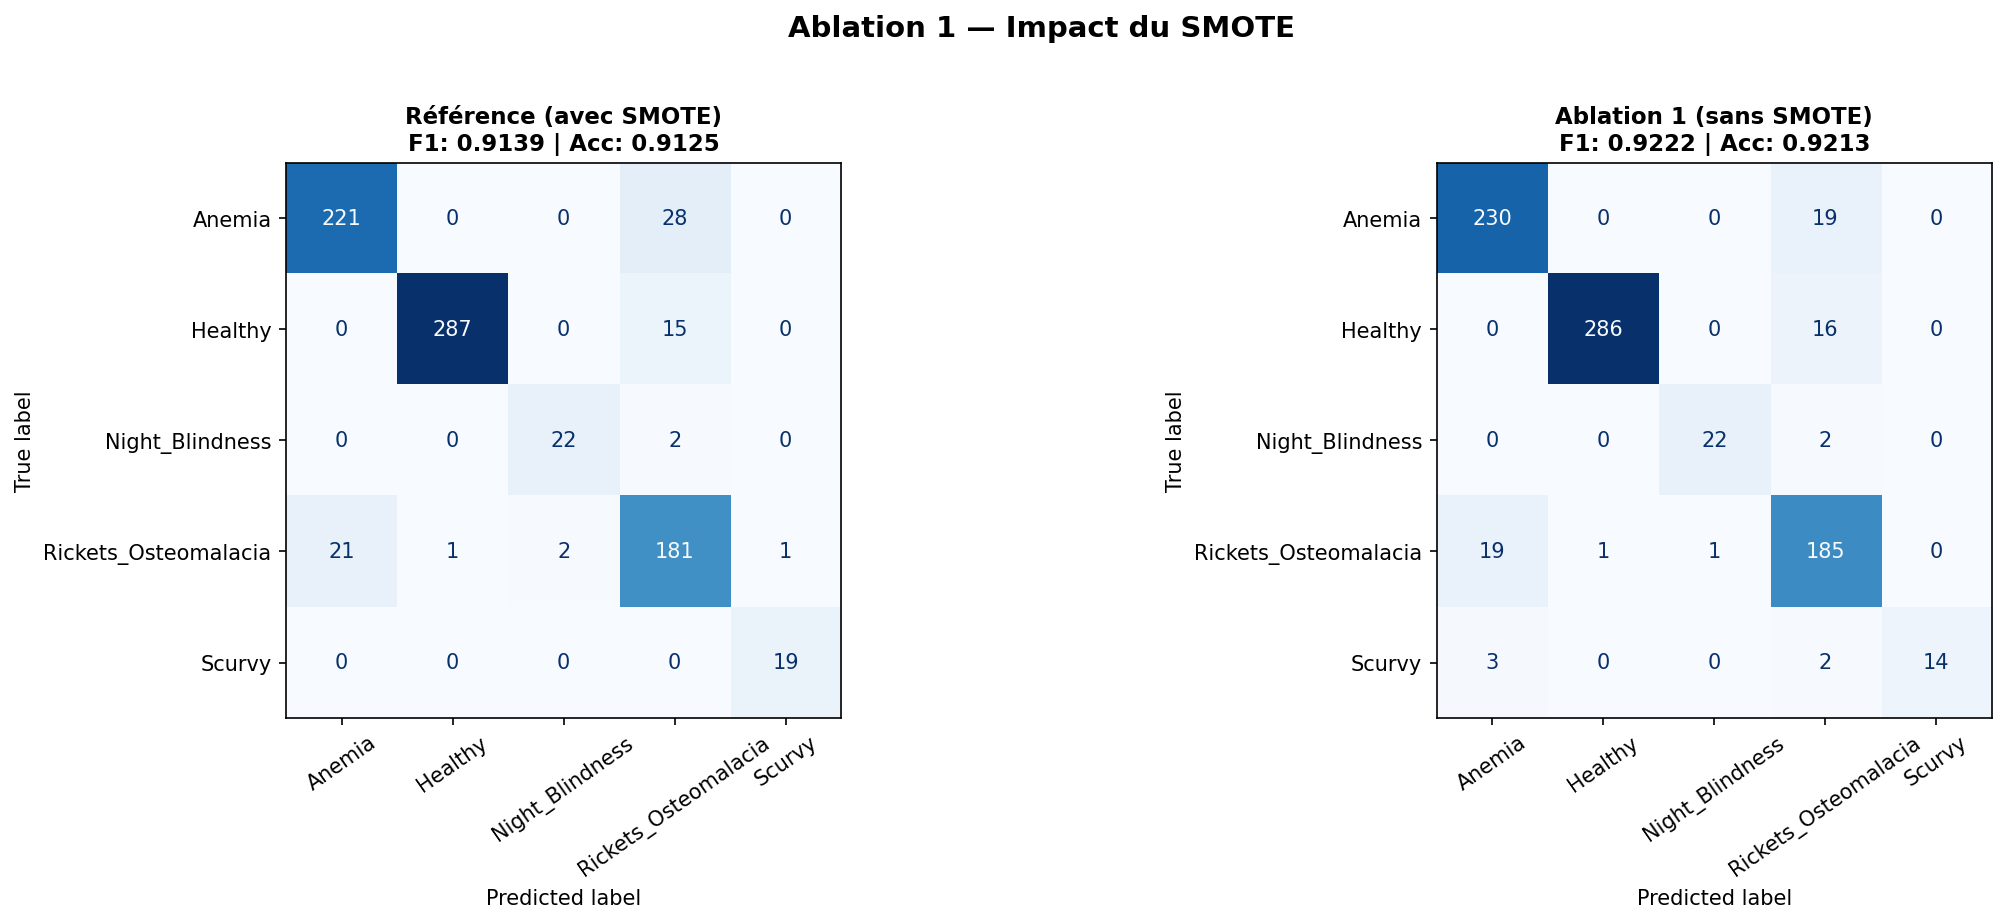
\includegraphics[width=0.80\linewidth]{ablation1_smote.png}
    \caption{Comparaison avec/sans SMOTE}
\end{figure}

\section{Ablation 2 — Impact des variables lifestyle}
\label{ann:abl2}
\begin{figure}[H]
    \centering
    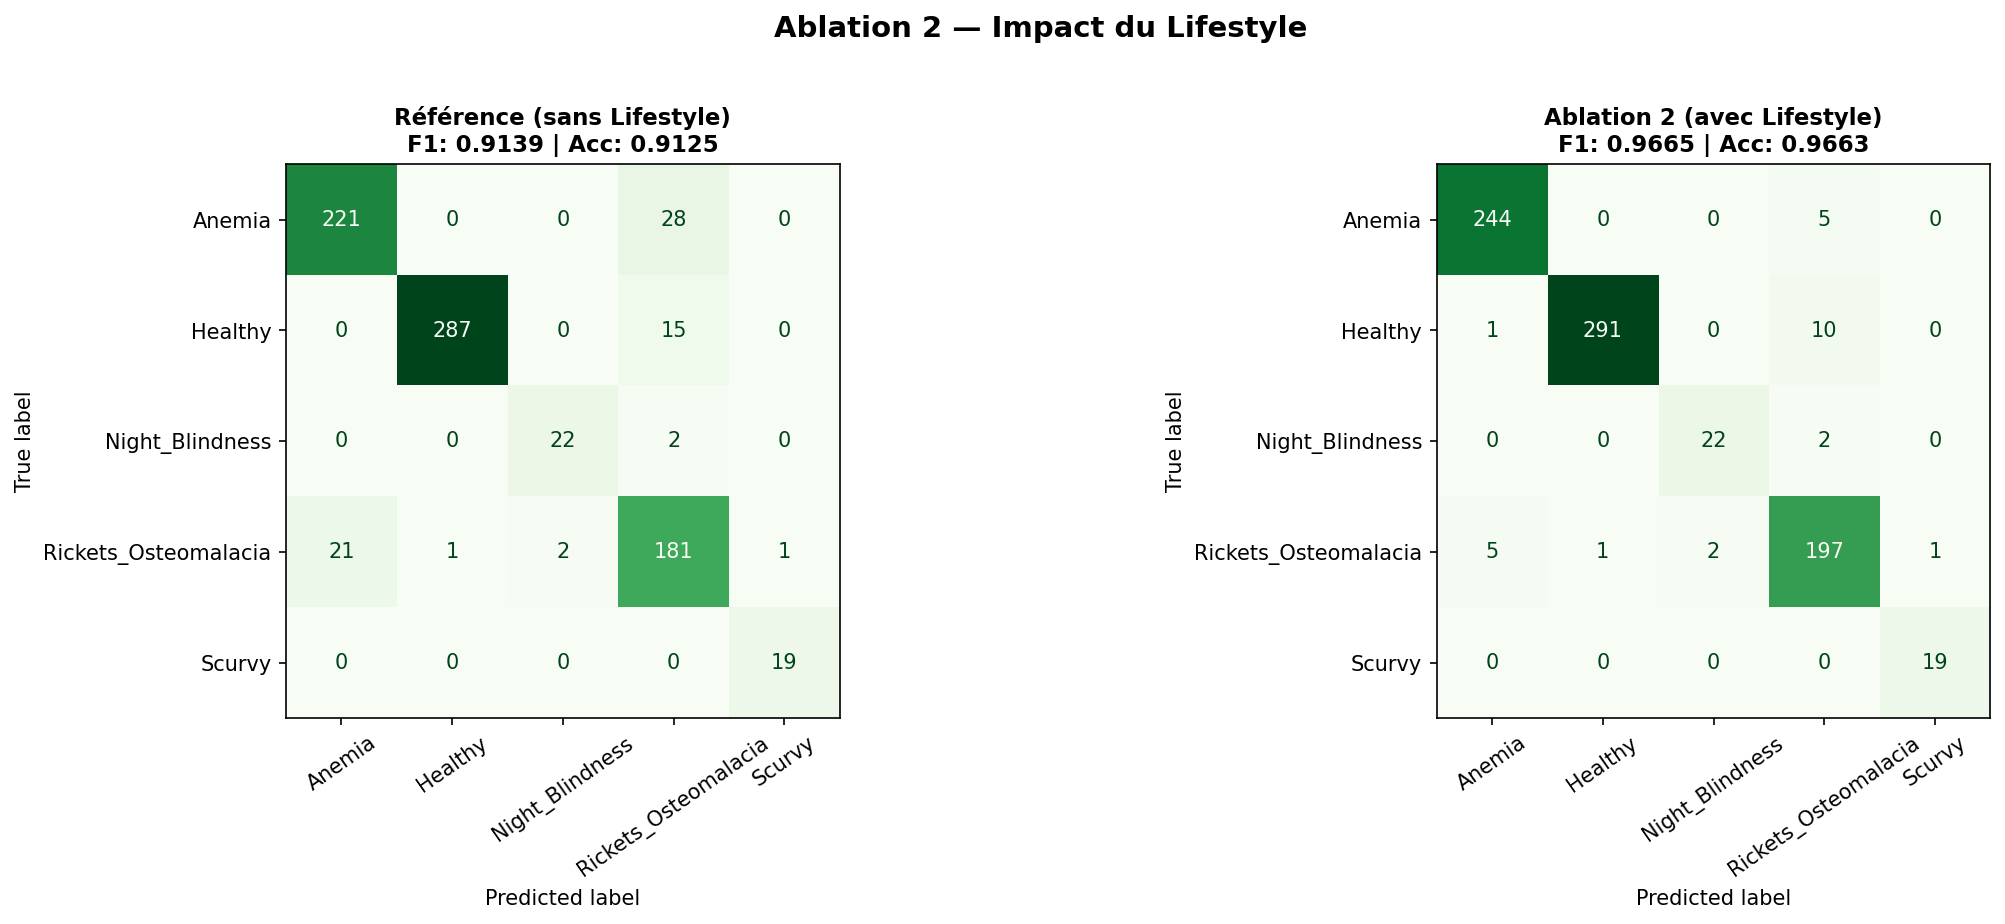
\includegraphics[width=0.80\linewidth]{ablation2_lifestyle.png}
    \caption{Gain apporté par les variables socio-comportementales (+5,3\,\% F1)}
\end{figure}

\section{Ablation 3 — Impact des biomarqueurs}
\label{ann:abl3}
\begin{figure}[H]
    \centering
    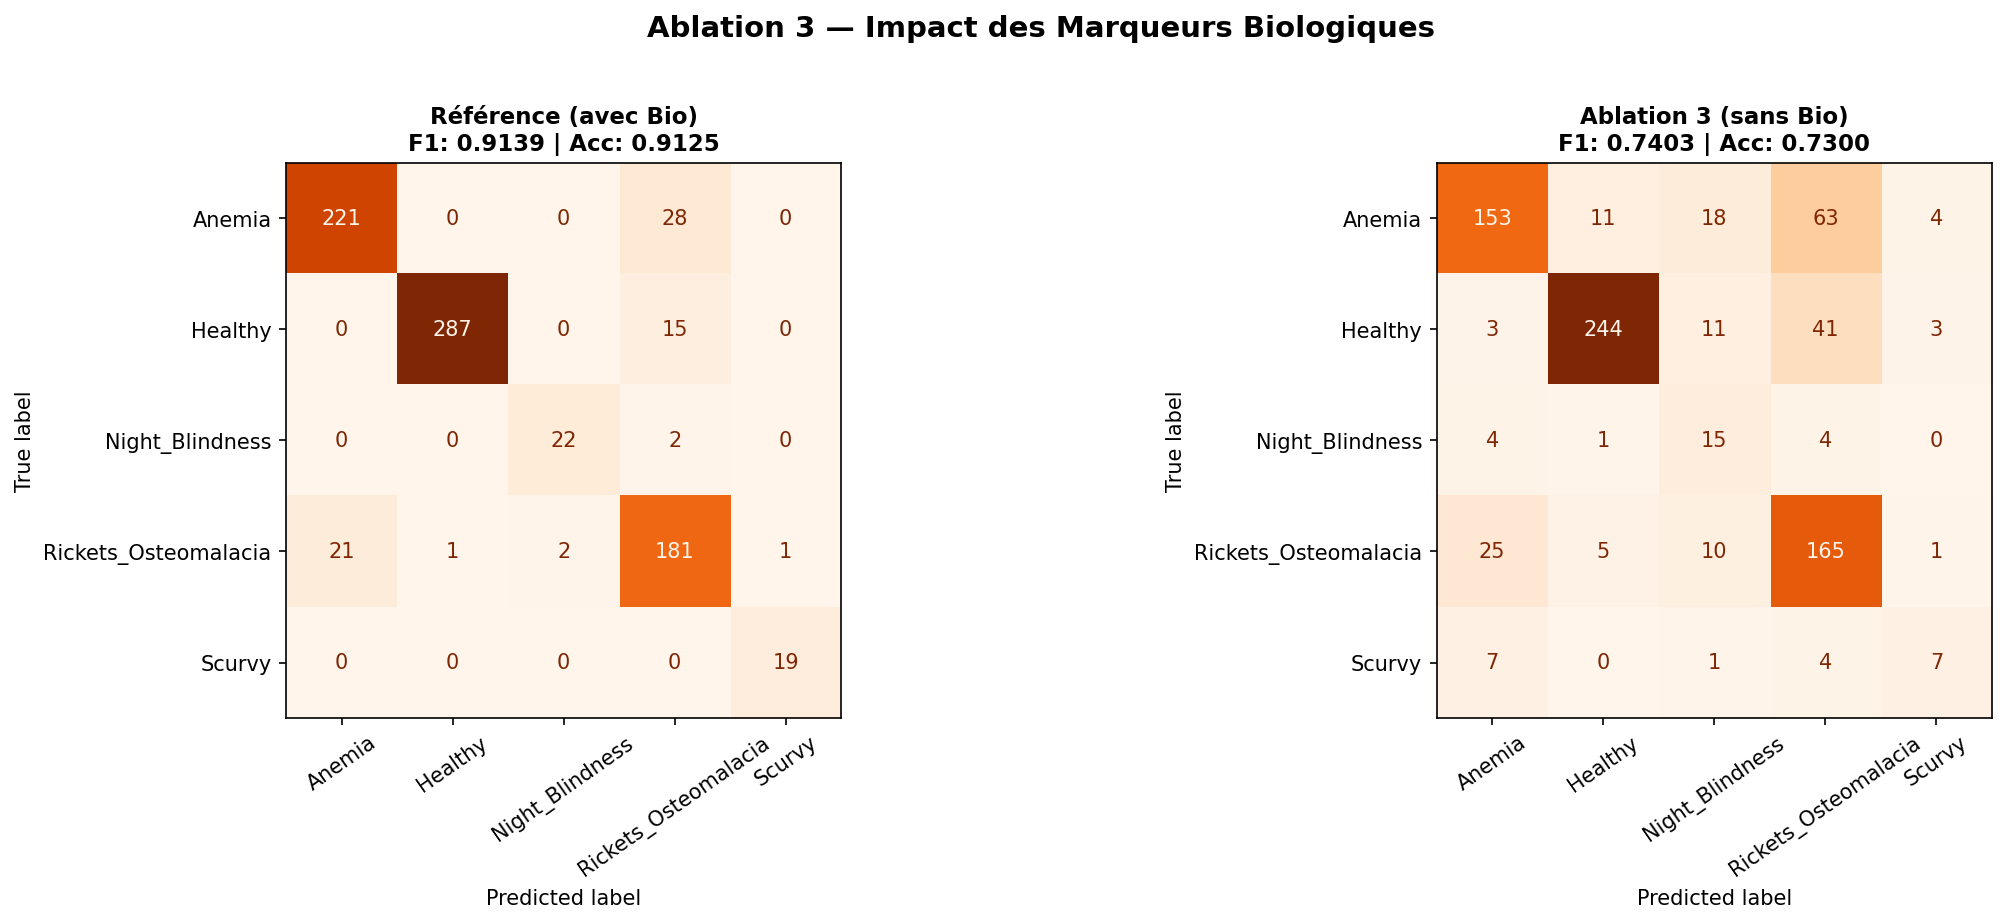
\includegraphics[width=0.80\linewidth]{ablation3_bio.png}
    \caption{Chute de performance sans biomarqueurs ($-$17,4\,\% F1)}
\end{figure}

\section{Ablation 4 — Impact de la normalisation}
\label{ann:abl4}
\begin{figure}[H]
    \centering
    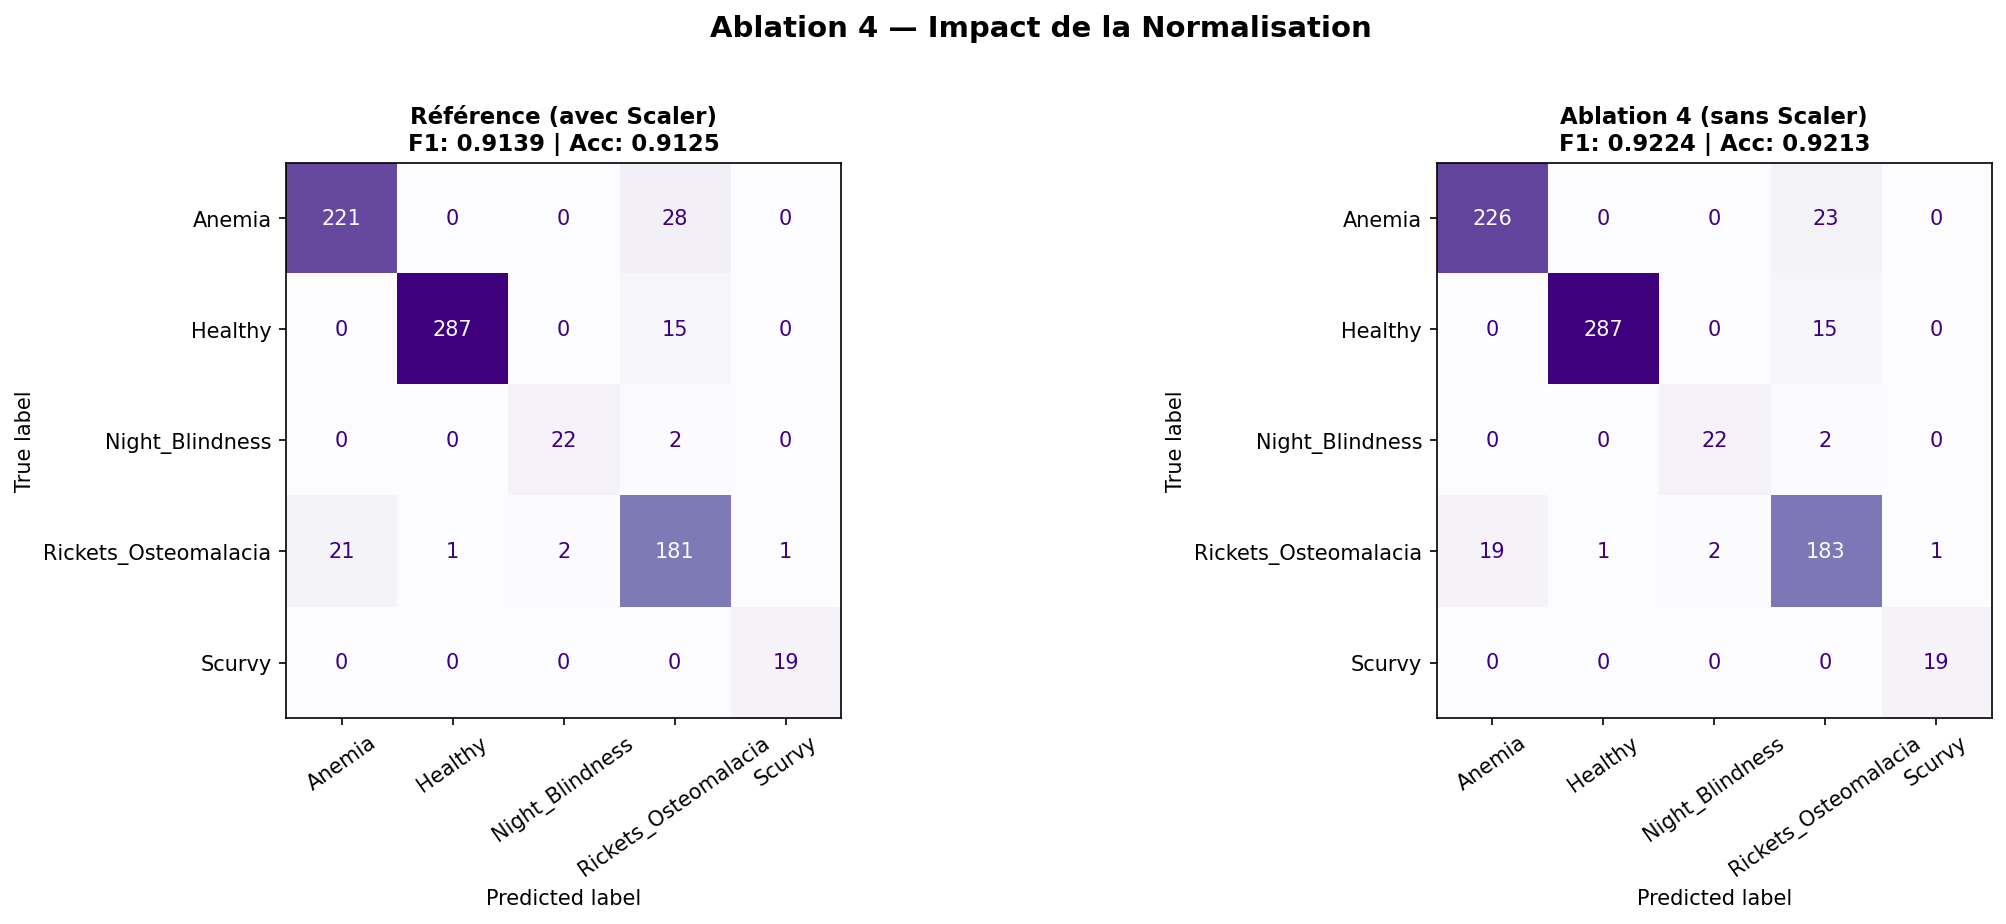
\includegraphics[width=0.80\linewidth]{ablation4_scaler.png}
    \caption{Comparaison avec/sans StandardScaler}
\end{figure}

\section{Récapitulatif de l'étude d'ablation}
\label{ann:abl_recap}
\begin{figure}[H]
    \centering
    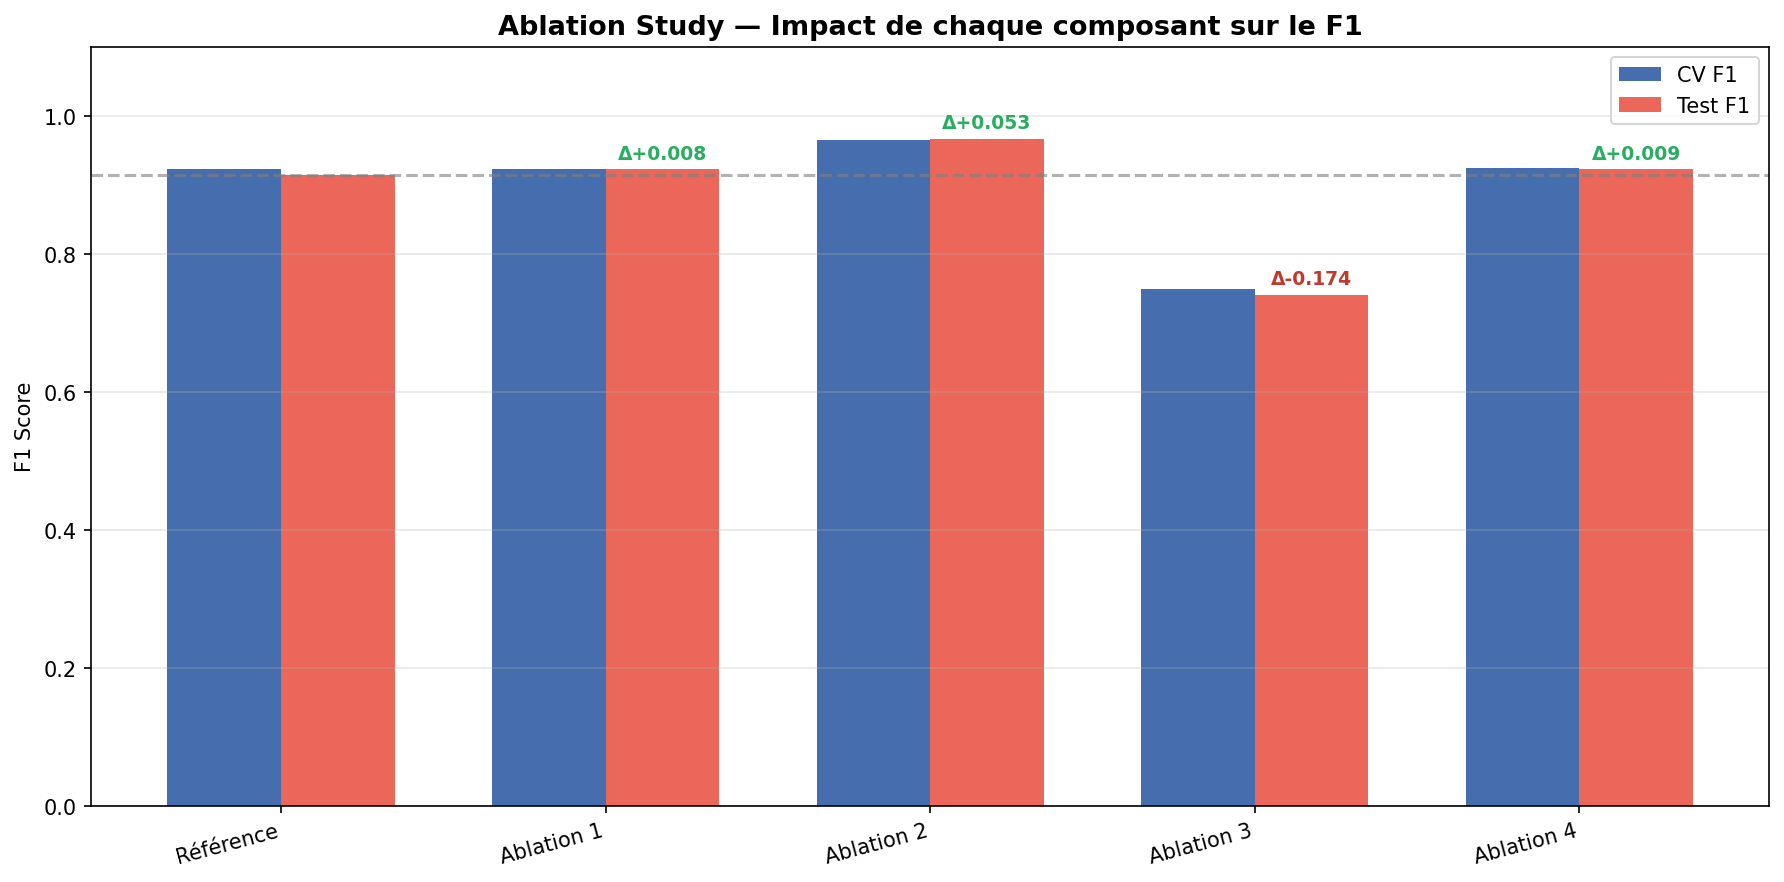
\includegraphics[width=0.80\linewidth]{ablation_recap_final.png}
    \caption{Synthèse des quatre ablations}
\end{figure}

\section{Matrice de confusion — Holdout final (v5)}
\label{ann:holdout_cm}
\begin{figure}[H]
    \centering
    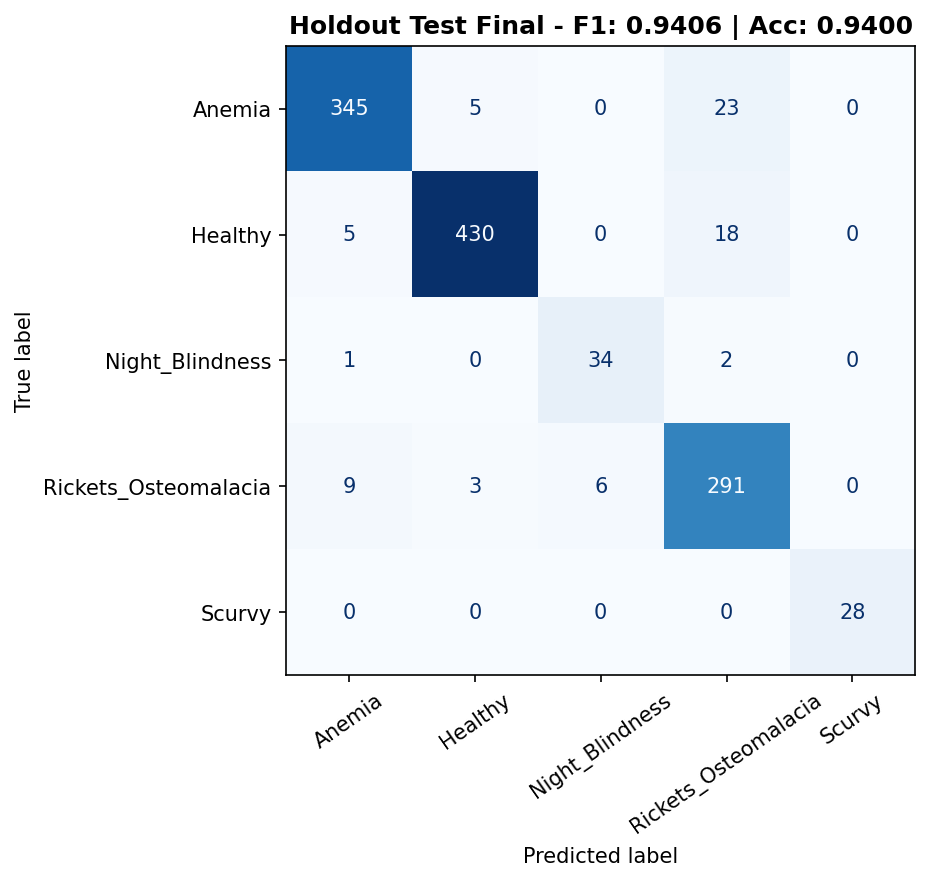
\includegraphics[width=0.70\linewidth]{holdout_confusion_matrix.png}
    \caption{Matrice de confusion sur le holdout ($n=1\,200$) --- F1 = 0,9406, Exactitude = 0,9400}
\end{figure}

\section{Matrices de confusion — Modèles v2 (comparaison RF/SVM/k-NN)}
\label{ann:conf_v2}
\begin{figure}[H]
    \centering
    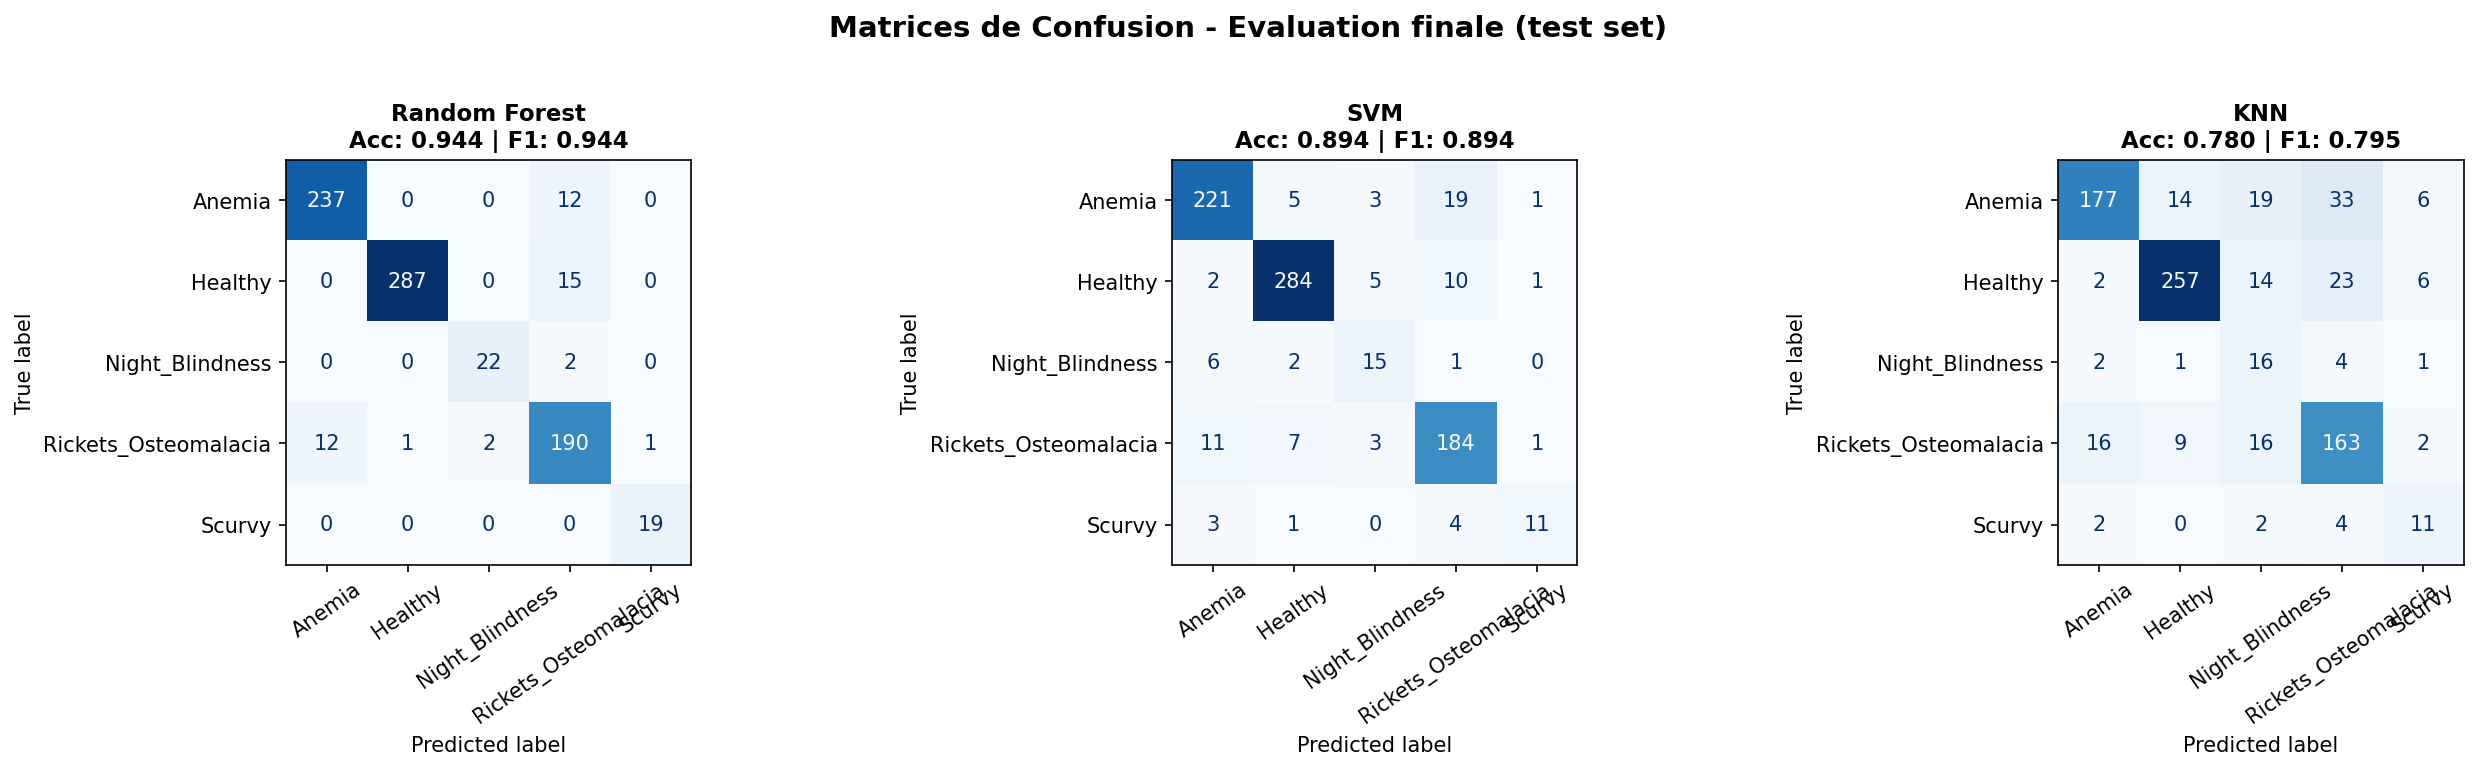
\includegraphics[width=\linewidth]{matrices_confusion_v2.png}
    \caption{Matrices de confusion des trois modèles --- version 2}
\end{figure}

\section{Comparaison globale des modèles}
\label{ann:comparaison}
\begin{figure}[H]
    \centering
    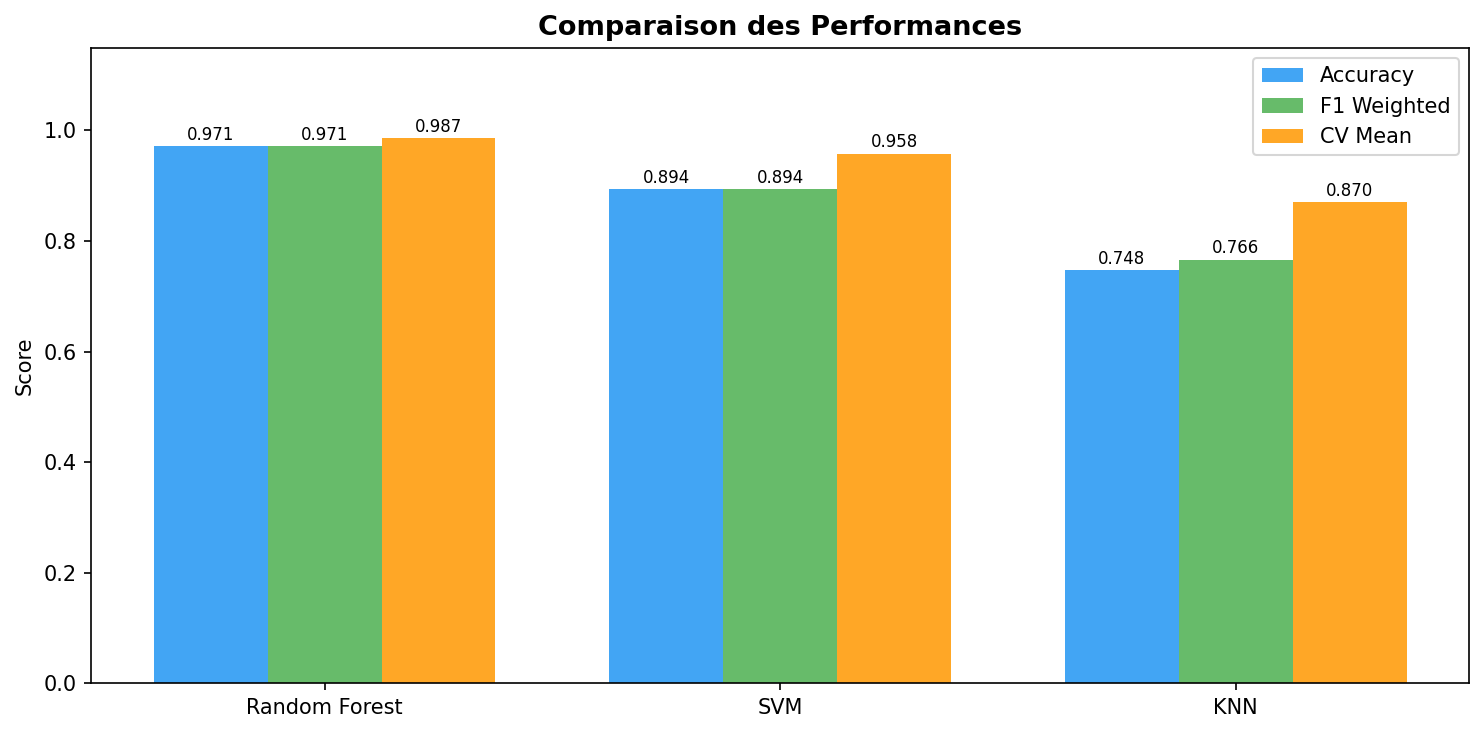
\includegraphics[width=0.75\linewidth]{comparaison_modeles.png}
    \caption{Comparaison F1 validation croisée vs test (RF, SVM, k-NN)}
\end{figure}

\section{Importance des variables}
\label{ann:feat_imp}
\begin{figure}[H]
    \centering
    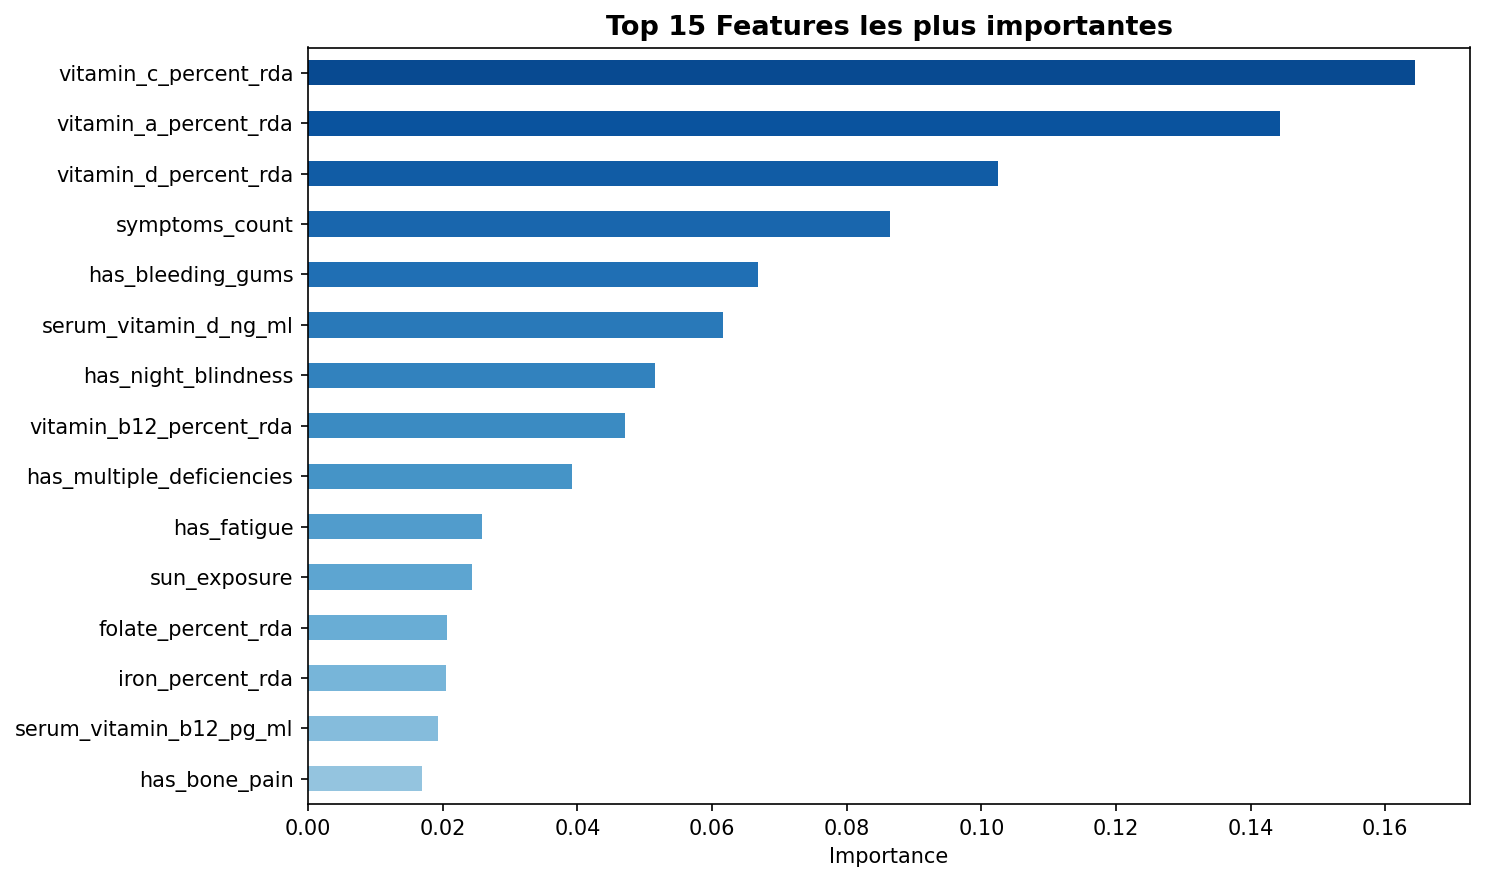
\includegraphics[width=0.80\linewidth]{feature_importance.png}
    \caption{Importance des variables --- Random Forest version intermédiaire
        (21 variables, sans lifestyle). Le classement diffère du modèle final
        v5 (Table~\ref{tab:feat_imp}) qui intègre les 10 variables
        socio-comportementales supplémentaires.}
\end{figure}

\section{Courbes d'apprentissage}
\label{ann:learning}
\begin{figure}[H]
    \centering
    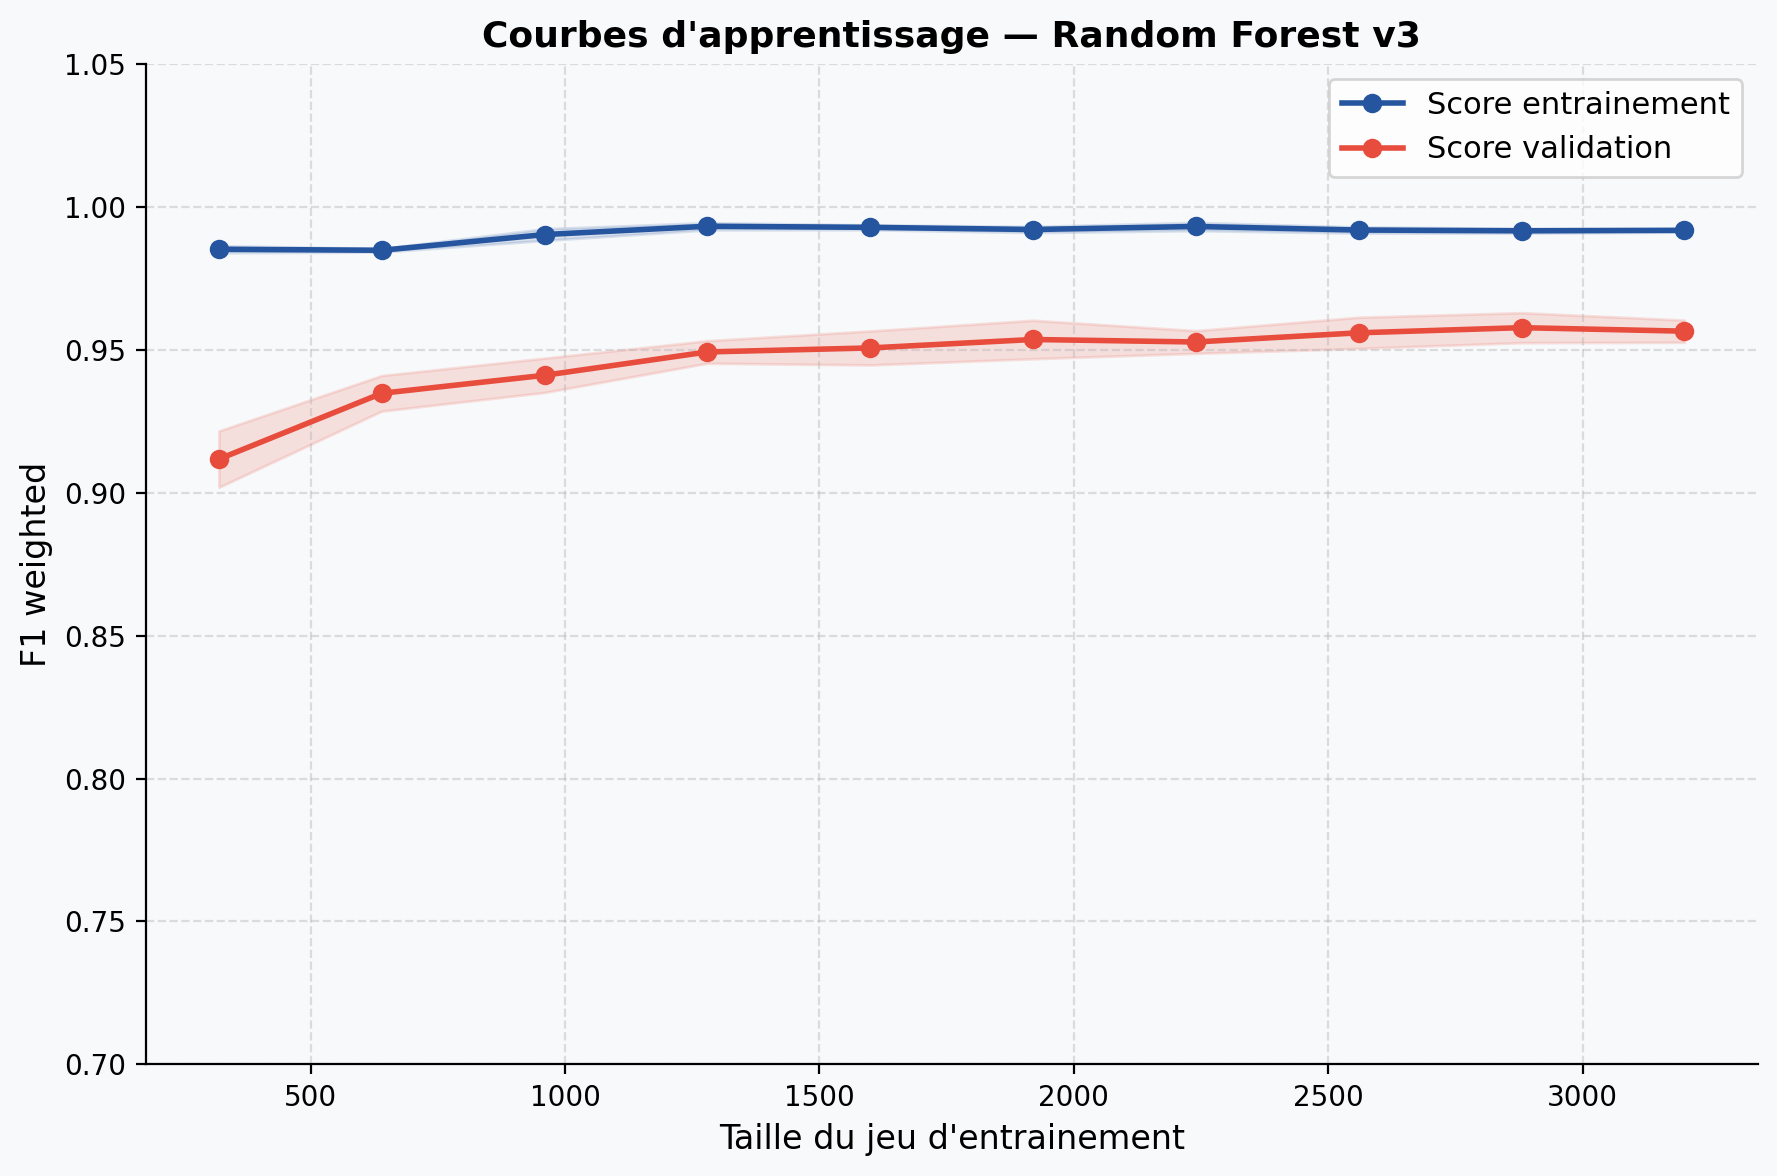
\includegraphics[width=0.80\linewidth]{learning_curves_v3.png}
    \caption{Courbes d'apprentissage --- F1 entraînement vs validation (RF v3)}
\end{figure}

\section{Courbes ROC (One-vs-Rest)}
\label{ann:roc}
\begin{figure}[H]
    \centering
    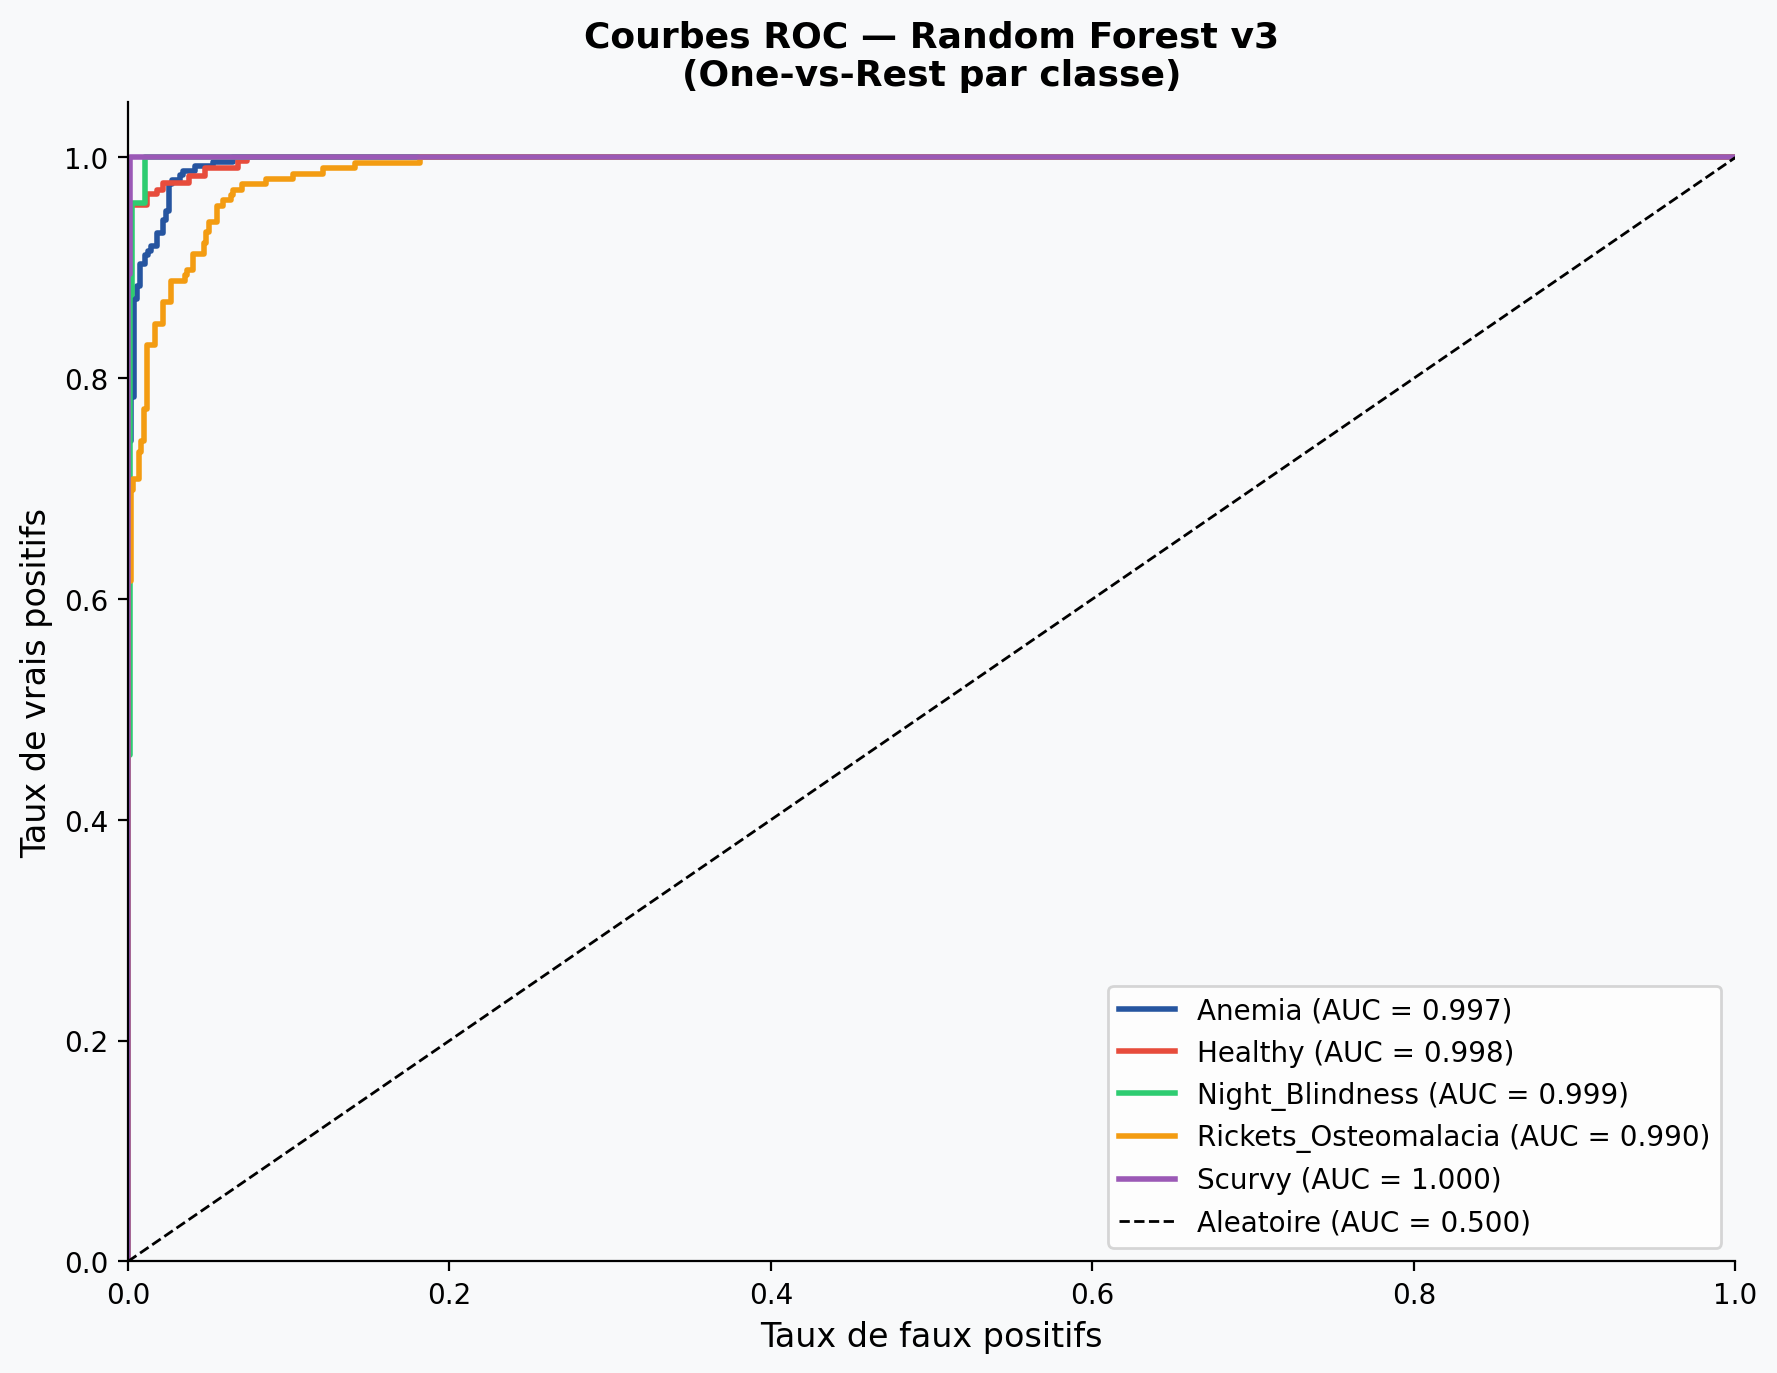
\includegraphics[width=0.80\linewidth]{roc_curves_v3.png}
    \caption{Courbes ROC par classe --- Random Forest v3 (AUC $>$ 0,95 pour toutes les classes)}
\end{figure}

\end{document}
